\documentclass[10pt]{report}

%% Text-Encoding festlegen. Mit utf8 oder utf8x funktionieren Umlaute wie gewohnt.
%% (mit Bibtex funktioniert nur utf8)
\usepackage[utf8x]{inputenc}

%% Sprachdatei für Trennregeln, Datum-Format und ähnliches festlegen
%\usepackage[german]{babel}  % nötig für Umlaute
\usepackage[ngerman, english]{babel}

%% optimiert das typographische Erscheinungsbild
\usepackage{microtype}

%% erlaubt Listen einfacher zu formatieren (bietet nosep für kompakte Listen)
\usepackage{enumitem}
%% erlaubt hübsche Tabellen über mehrere Seiten, beinhaltet booktabs (\toprule, \midrule, ...)
\usepackage{ctable}
%% ermöglicht farbigen Text ({\color{red} ...})
\usepackage{xcolor} 


\usepackage{mathrsfs}

%% erweiterte Funktionalität für Formeln (Pakete der American Mathematical Society)
\usepackage{amsfonts,amsmath,amsthm,amssymb}
 \numberwithin{equation}{chapter}

%% vordefinierte Einheiten, einfaches Angeben von Einheiten (\SI{8 \pm 1}{cm})
%%   die Unsicherheit soll mit +- abgetrennt werden
\usepackage[separate-uncertainty]{siunitx}
\sisetup{
    range-units = single,       % \SIrange soll die Einheit nur einmal anzeigen
    list-units  = repeat,       % \SIlist soll die Einheit wiederholen
}
%% bei siuntix funktioniert babel leider nicht
%% für englische Dokumente sollten diese Zeilen auskommentiert werden. 
\sisetup{
    range-phrase         = { bis },
    list-final-separator = { und },
%    list-pair-separator  = { und }, % an Uni noch nicht verfügbar
}

%% erlaubt es Bilddateien einzubinden
%% (ctable graphicx intern auch. Trotzdem ist es sinnvoll graphicx expilizt zu laden.
%%  Sonst entstehen schwehr verständliche Fehler, wenn ctable entfernt wird)
\usepackage{graphicx}
%% ermöglicht Bilder und Tabellen am eingegebenen Ort zu platzieren ([H])
\usepackage{float}
%% ermöglicht Unter-Bilder in einer figure-Umgebung
\usepackage{caption}
\captionsetup[figure]{font=footnotesize, labelfont=bf}
\captionsetup[subfigure]{labelformat=parens, labelsep=space, font=small}

\usepackage{subfig}
%% Grafik-Dateien werden in den folgenden Ordnern gesucht
\graphicspath{{img/}}
%% Grafikdateien haben die folgenden Endungen (höchste Priorität zu erst)
\DeclareGraphicsExtensions{.pdf,.png,.jpg}

%% Vertikaler Abstand zwischen Absätzen, Beginn eines Absatzes nicht einrücken
\usepackage{parskip}
% \setlength{\parskip}{0.6em}   % Vertikaler Abstand zwischen Absätzen anpassen 
% \setlength{\parindent}{0em}   % Einrück-Abstand anpassen 

%% zeige Labels im Seitenrand. Dies ist praktisch um Verweise zu kontrollieren
\usepackage[final]{showkeys} % die Option 'final' deaktiviert die Ausgabe von showkeys

\linespread{1.3}	% 1.3

%% Seiten-Layout einstellen
\usepackage[
 a4paper,
 total={13.8cm,21.7cm},          % Breite und Höhe des Inhalt-Bereichs
 top=40mm, left=36mm,        % Ränder oben und links
 headsep=10mm,               % Abstand des unteren Rands der Kopfzeile vom oberen Rand des Inhalts
 footskip=10mm               % Abstand des unteren des Inhalts zum oberen Rand der Fusszeile
% showframe					 % for troubleshooting
]{geometry}

%% Ermöglicht Links im PDF 
%%   sollte möglichst spät in der Präambel geladen werden
\usepackage[
 pdftex,                        % wir verwenden pdftex/pdflatex
 bookmarks=true,                % wir wollen auch im PDF-Reader ein Inhaltsverzeichnis
 bookmarksdepth=3,              % das Inhaltsverzeichnis soll 3 Tiefen enthalten
 colorlinks=true,               % Linktexte sollen Farbig sein 
 linkcolor=black,               % Links innerhalb des Dokuments bleiben schwarz
 citecolor=black,               % Links zu Quellenangaben bleiben ebenfalls schwarz
 urlcolor=black,                 % URL-Linktexte sollen blau dargestellt werden
%  pdfborder={0 0 0}              % Links im PDF erhalten keinen Rahmen, nur nötig wenn colorlinks=false
]{hyperref}

\usepackage{mathtools}

%% Angaben für die PDF-Eigenschaften
\hypersetup{
  pdfauthor = {Kevin Hauser},
  pdftitle = {QM1 - Zusamenfassung},
  pdfsubject = {LaTeX},
  pdfkeywords = {LaTeX, Beispiel}
}



%% definiert \cref: Referenzen mit korrekter Bezeichnung (z.B. "Abbildung 1")
%%   die Nummer alleine ist weiter mittels \ref verfügbar
%% muss NACH 'hyperref' geladen werden
%\usepackage[german]{cleveref}
\usepackage[english, capitalise]{cleveref}


%================  for subfigure


%%%%%%%%%%%%%%%%%  additional libraries

% link: http://tex.stackexchange.com/questions/36524/how-to-put-a-framed-box-around-text-math-environment
\usepackage{mdframed}
\usepackage{lipsum} % for creating dummy text

\mdfdefinestyle{MyFrame}{%
    linecolor=black,
    outerlinewidth=2pt,
    roundcorner=20pt,
    innertopmargin=\baselineskip,
    innerbottommargin=\baselineskip,
%	leftmargin=1cm,
    innerrightmargin=20pt,
    innerleftmargin=20pt,
    backgroundcolor=gray!10!white,
    frametitlerule =true,
%    frametitlerulewidth=0.5pt,
	frametitlerulecolor=black
    }
    
    
\usepackage{physics}

\usepackage{siunitx}	% for typeset SI units correctly
    

%=======================================================================
% new commands
%=======================================================================

\newcommand{\myRef}[1]{
  Fig.\ref{#1}
}

\newcommand{\myEq}[1]{
  Eq.\ref{#1}
}

%\newcommand{\Tc}{
%  $T_c$
%}
%\newcommand{\lsco}[1][]{
%  LSCO#1
%}
%
\newcommand*{\NewPage}{
  \newpage\null\thispagestyle{empty}\newpage
}

\newcommand{\refEq}[1]{
  Eq  \ref{#1}
}

\DeclareMathOperator{\sign}{sign}

%========================================================================================================
%========================================================================================================
% Document
%========================================================================================================
%========================================================================================================

%% Angaben für \maketitle
\title{BA - rough sketch}
\author{Kevin Hauser}
% \date{7. Mai 2013}             % ohne Angabe wird das heutig Datum verwendet

\begin{document}
\pagenumbering{roman} %
%=======================================================================
% Title page
%=======================================================================

\begin{titlepage}
    \begin{center}
%        \vspace*{1cm}
       
        \Huge
        \textbf{Mitschrift KOMA}
       
        \vspace{0.5cm}
        \Large

%        \includegraphics[width=0.4\textwidth]{{{img\manipulator.png}}}
 
 		\vspace{3.0cm}
		\begin{figure}[H]
 		\centering
 		
\includegraphics[width=0.5\textwidth]{{{../img/uzh_logo}}}
		\end{figure} 

       
        \vspace{1cm}
       
        %A thesis presented for the degree of\\
        %Doctor of Philosophy
       
       

       
       
        \vspace{1.5cm}
       
        Department of Physics\\
        University of Zurich\\
        \today
       
    \end{center}
\end{titlepage}


% empty page
\null
\thispagestyle{empty}
\setcounter{page}{2}


%=======================================================================
% Introduction
%=======================================================================


\begin{abstract}



\setcounter{page}{3}
\end{abstract}

\setcounter{page}{4}
\NewPage
\setcounter{page}{5}

\tableofcontents
\thispagestyle{empty} % don't show (roman) page number on titlepage

%=======================================================================
% Charge Order
%=======================================================================

\chapter{Charge Order}
\pagenumbering{arabic}

\section{Peierl Transition}


\section{From Causality to Kramer-Kronig relation}


Looking at a causal function $\tilde{\chi}(t)$, we can split it, like every analytical function, in an even $\chi_{even}(t)$ and an odd $\chi_{odd}(t)$ part.


\begin{minipage}{0.45\textwidth}
  \begin{equation*}
    \tilde{\chi}(t) ~~ = ~~ \left\{ \begin{array}{lc} 
      0        &  t < t_0 \\
      \chi(t)  &  t > t_0
    \end{array}\right.
  \end{equation*}
%   
\includegraphics[width=0.8\textwidth]{img/uzh_logo}
\end{minipage}
\begin{minipage}{0.1\textwidth}
\end{minipage}
\begin{minipage}{0.45\textwidth}
   
\includegraphics[width=0.8\textwidth]{../img/uzh_logo}
\end{minipage}

%Every function $\tilde{\chi}(t)$ can be divided in an even $\chi_{even}(t)$ and an odd $\chi_{odd}(t)$ part.

\begin{equation} \label{eq:even_odd}
\tilde{\chi}(t) ~~ = ~~ \frac{\tilde{\chi}(t) + \tilde{\chi}(-t)}{2} + \frac{\tilde{\chi}(t) - \tilde{\chi}(-t)}{2} ~~ = ~~ \chi_{even}(t) + \chi_{odd}(t)
\end{equation}


Multiplying the even part of this function with the signum function yields,

\begin{equation}
  \sign(t) \cdot \chi_{even} ~~ = ~~ \sign(t) \cdot \left\{ \frac{\tilde{\chi}(t)}{2} + \frac{\tilde{\chi}(-t)}{2} \right\} ~~ = ~~~\frac{\tilde{\chi}(t)}{2} - \frac{\tilde{\chi}(t)}{2} ~~ = ~~ \chi_{odd}(t)
\end{equation}


Using this relation to replace $\chi_{odd}(t)$ in \refEq{eq:even_odd}.


\begin{equation}
\tilde{\chi}(t) ~~ = ~~ \chi_{eve} + \chi_{odd} ~~ = ~~ (1 + \sign(t)) \cdot \chi_{even}(t) ~~ = ~~ \sigma(t) \cdot \chi_{even}(t)
\end{equation}

%=======================================================================
% 
%=======================================================================

\subsubsection{Onsager Relation}

\begin{equation}
  S \cdot \left( \frac{1}{B_{n+1}} ~-~ \frac{1}{B_n} \right) ~~=~~ \frac{2 \pi e}{\hbar}
\end{equation}

$S$ is the Fermi surface ($S=\pi k_F^2$.

\begin{equation}
  F ~~\equiv~~ \left( \frac{1}{B_{n+1}} ~-~ \frac{1}{B_n} \right)^{-1}
\end{equation}

\begin{equation}
  F ~~=~~ \frac{\Phi_0}{2 \pi^2} \cdot S
\end{equation}

where $\Phi_0 = \frac{h}{2e} = \text{Flux Quantum}$



%=======================================================================
% Second quantization
%=======================================================================
%
% lec.notes 10.10.17 - first part
% lec-notes 16.10.17 - second part

\subsubsection{Second quantisation: Free electron gas} % 10.10.17 - first part

Hamiltonian of a free electron gas can be written as. 

\begin{equation}
  H ~~=~~ \sum_{k \sigma} \frac{(\hbar \hat{k})^2}{2m} c_{k \sigma}^\dag c_{k \sigma}
\end{equation}


The ground state at $T=0K$ is create by applying the electron-creation operators $c_{k_i \uparrow}$ of the $i-\text{th}$ electron $e_{i \uparrow}$ to the vacuum state $|0\rangle$ for every electron that is present in the electron gas. 

\begin{equation}
  | \text{FS} \rangle ~~=~~ c_{k_{N/2} \uparrow} c_{k_{N/2} \downarrow} ... c_{k_1 \uparrow} c_{k_1 \downarrow} | 0 \rangle ~~=~~   
\end{equation}

To get the total number of electrons $N$ the number operator $\hat{N} = \sum_{k \sigma} c_{k\sigma}^\dag c_{k\sigma}$ can be applied on the ground state to the ground state $| \text{FS} \rangle$

\begin{equation}
  N ~~=~~ \langle \text{FS} | \hat{N} | \text{FS} \rangle 
    ~~=~~ \langle \text{FS} | \sum_{k\sigma} c_{k\sigma}^\dag c_{k\sigma} | \text{FS} \rangle
\end{equation} 

This expression is equivalent to a step function 



\subsubsection*{Second Quantization: Free Electron Gas} % 16.10.17 - second part 

$ k_F^3 = 3 \pi^2 n$

$ E_0 = \frac{3}{5} N epsilon_F$

Bohr Radius: $a_0 = \frac{\hbar}{m e^2}$

\begin{equation*}
\frac{3 \pi^2}{k_F^3} ~~ = ~~ \frac{1}{n} ~~ = ~~ \frac{V}{N} ~~ = ~~ \frac{4\pi}{3} \left(r_S a_0 \right)^3 ~~~~ \Rightarrow ~~~~ r_S = \left( \frac{9\pi}{4} \right)^{1/3} \frac{1}{a_0 k_F}
\end{equation*}

\begin{equation*}
\frac{E_0}{N} ~~ = ~~ \frac{2.21}{r_S^2} \frac{e^2}{2a_0}
\end{equation*}



\subsubsection*{Electron Interaction}

\begin{equation*}
  \frac{E_1}{N} ~~ = ~~ \frac{\bra{FS} V_{el-el} \ket{FS}}{N} ~~ = ~~ 
  - \frac{e^2}{2} \frac{V}{N} \frac{k_F^4}{2 \pi^3} ~~=~~ - \frac{0.916}{r_S} \frac{e^2}{2 a_0}
\end{equation*}


\textcolor{red}{plot - energy minimum at $r_S$}


\begin{equation}
  V_\text{el-el} ~~=~~ \frac{1}{2V} \sum_{\sigma_1 \sigma_2} \sum_{k_1 k_2 q} 
    V_q c_{k_1+q}^\dag c_{k_2-q}^\dag c_{k_2} c_{k_1}
\end{equation}


\subsubsection{Electron Tight Binding Model}
% lec-notes 17.10.17





%=======================================================================
% Magnetism
%=======================================================================

\chapter{Magnetism}

\section{Paramagnetism}

\subsubsection{Magnetic Moment}

\textcolor{red}{insert picture - magnetic moment}

If $\vec{A}$ is the area inside the loop and $I$ the current, the magnetic moment can be written as

\begin{equation} \label{eq:mag_mom}
  \vec{\mu} ~~=~~ I \vec{A}
\end{equation}


\subsubsection{Example: Hydrogen Atom}

\textcolor{red}{insert picture - hydrogen atom and orbiting electron}

The magnetic moment of a hydrogen atom can be described semi-classically by assuming the electron to be on a fixed trajectory orbiting the hydrogen nucleus with constant radius $r$ and velocity $v$. The current $I$ produced by the moving electron can be written as $I = -e/\tau$ with the orbital period $\tau = 2\pi r/v$. For the loop area we use the formula $A= \pi r^2$. This leads the magnetic moment to be

\begin{equation} \label{eq:dev_mag_mom}
  \mu ~~=~~ \frac{-e v \pi r^2}{2 \pi r} ~~=~~ \frac{-evr}{2} ~~=~~ \frac{-e m v r}{2m}
\end{equation}

We can identify the classical definition of the angular momentum  $\vec{l} = \vec{r} \times m \vec{v}$ in the numerator. Taking the quantisation of angular momentum $|\hat{l}| = n \hbar$ in quantum mechanics into account we can rewritte expression \ref{eq:dev_mag_mom} for $n=1$

\begin{equation} \label{eq:bohr_mag}
  \mu ~≃ ~~ \frac{-e \hbar}{2m} ~~ \equiv ~~ -\mu_B
\end{equation}

Which we define as the Bohr magneton $\mu_B$.


\subsubsection{Magnetic Moment of Atoms}

The total angular momentum in an atom is given as the sum of total orbital angular Momentum $\hat{L}$  and total spin angular momentum $\hat{S}$

\begin{equation}
  \hat{J} ~~≃~~ \hat{L} ~+~ \hat{S}
\end{equation}

\subsubsection{Magnetisation}

Considering a solid with $N$ atoms each having a magnetic moment $\vec{\mu}$. We define the magnetization as 

\begin{equation}
  \vec{M} ~~\equiv~~ \frac{\text{Magnetic moment}}{\text{Volume}}
\end{equation}

\begin{figure}
  \centering
  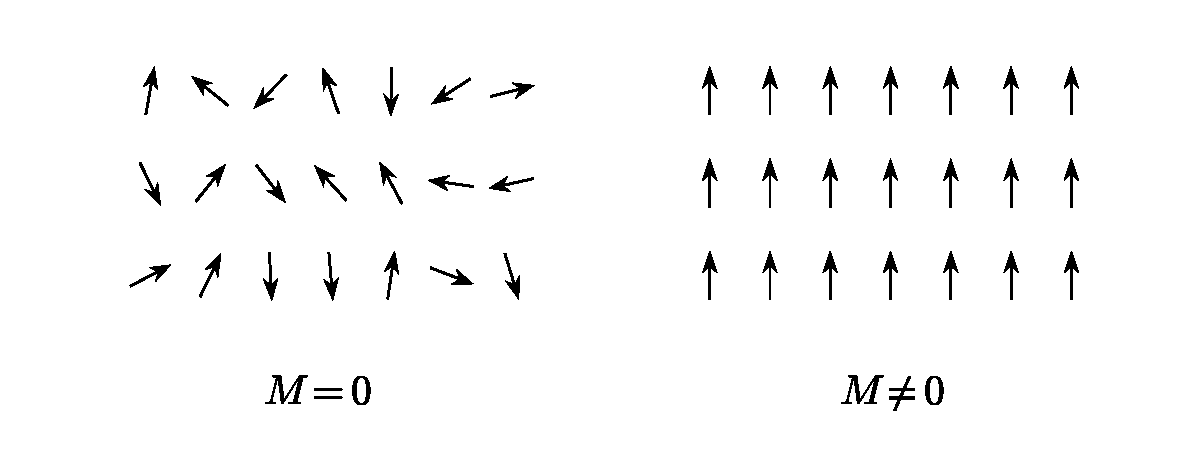
\includegraphics[width=0.8\linewidth]{../img/mag_in_solid.pdf}
  \caption{hohohoh}
\end{figure}

\subsubsection{Magnetic Moment in a $\vec{B}$-Field}


From classical electrodynamics we know that the potential energy $E$ of a magnetic moment $\vec{\mu}$ in a magnetic field $\vec{B}$ is described as

\begin{equation}
  E ~~=~~ - \vec{\mu} ~\cdot~ \vec{B}
\end{equation}

To get a feeling for the order of magnitudes of magnetic energy of atomic scale we 

\begin{equation*}
  \mu_B ~\times~ 1 \text{Tesla} ~~\simeq~~ \SI{0.05}{meV}
\end{equation*}

This is comparable to the energy one has to put into a system to increase its temperature by \SI[mode=text]{1}{K} ($ k_B \cdot \SI{1}{K} ~~\simeq~~ \SI{0.084}{meV}$).


\subsubsection{Magnetic susceptibility}

\begin{equation} \label{eq:mag_suscept}
  \chi ~~≃~~ \frac{\mu_0 \vec{M}}{\vec{B}}
\end{equation}

We can look at the magnetic susceptibility $\chi$ as response function. $\chi$ describes the response of the system $\vec{M}$ when exposed to an external changing field $\vec{B}$.
To simplify things in the calculations we will make the following constraints on $\vec{B}$.

\begin{align*}
  \vec{B} \text{is static} ~~~~ &  \Rightarrow  ~~~~ \text{no time dependence}\\
  \vec{B} \text{is homogeneous} ~~~~ & \Rightarrow  ~~~~ \text{no depencence on}\ \vec{r}
\end{align*}


The definition of the susceptibility allows us now to classify materials depending on how the respond to an external magnetic field. We calc materials to be \textit{paramagnetic} if they align there spin parallel to the applied $\vec{B}$-Field. This is the case if $\chi > 0$. On the contrary we refer to materials as \textit{diamagnetic} if their inner magnetic moments align anti-parallel in respect to an applied field $\vec{B}$. This results in a negativ value for the susceptibility $\chi < 0$.

In reality, the response of systems is composed of multiple differenent responses which can have different origins.

\begin{equation}
  \chi_{total} ~~≃~~ \chi_\text{paramagnetic} ~+~ \chi_\text{diamagnetic} ~+~ ...
\end{equation}

Paramagnetism and diamagnetism can also have different origins. For example:

\begin{align*}
  \chi_\text{paramagnetic} ~~& ≃~~ \chi_\text{Langevin} ~+~ \chi_\text{Van Vleck} ~+~ \chi_\text{Pauli} ~+~ ....\\
  \chi_\text{diamagnetic} ~~& ≃~~ \chi_\text{electronic} ~+~ \chi_{superconductivity} ~+~ ...  
\end{align*}



\subsubsection{Diamagnetism}

\textcolor{red}{insert picture - loop current to illustrate lens law}

To symbolize diamagnetic behaviour we recall lens law. It states, that a a changing magnetic field induces a current which creates for itself a magnetic field that points in the opposit direction as the initial magnetic field change. In that way the system tries to compensate the externaly induced field changes.

To describe that, we use \ref{eq:mag_mom}, with the area $\vec{A} = \pi <r^2>$ and the current $I = -Z e/ \tau$ with the number of electrons $Z$ per atom and the orbit period $\tau$. expression the orbit period in terms of the \textit{cyclotron frequency} $\omega = eB/2m$ shows the dependency on the magnetic field.

\begin{equation}
  \tau ~~=~~ \frac{2\pi}{\omega} ~~=~~ \frac{4\pi m}{e B}
\end{equation}

Putting everything together we get the following expression to approximate the magnetic moment of a diamagnet

\begin{equation} \label{eq:mag_mom_diamag}
  \vec{\mu} ~~=~~ -\frac{Z e^2 B}{4\pi m} \pi <r^2> ~~=~~ -\frac{Ze^2B}{4m} <r^2>
\end{equation}

The magnetisation of a macroscopic material can be written as the sum over all the magnetic moments of its atoms resulting in

\begin{equation}
  \vec{M} ~~=~~ \mu_0 N \vec{\mu}
\end{equation}

where $N$ denotes the number of atoms per volume. Recalling \ref{eq:mag_suscept}, we find for the diamagnetic susceptibility caused by electrons

\textcolor{red}{compare formula with wikipedia. probably wrong by a prefactor}

\begin{equation}
  \chi_\text{Diamagnetic} ~~=~~ -\frac{\mu_0 N e^2 <r^2> Z}{4m}
\end{equation}


\subsubsection{Simplest Case: $e^-$ only}

Consider a system consisting of atoms with only one electron

\begin{equation}
  \rightarrow ~~ \hat{L} ~~=~~0, ~~~~ \hat{S} ~~≃~~ 1/2 ~~~~~~~~~\Rightarrow ~~ \hat{J} ~~=~~ 1/2
\end{equation}

Further more we asume for the spin g-factor $g \simeq 2$ (not proved). This system has only to states: \textit{spin-up} and \textit{spin-down}.


Consider the energy of these two states leads to

\begin{equation}
  E ~~=~~ - \vec{\mu} \cdot \vec{B} ~~=~~ \pm \mu_B \cdot |\vec{B}|
\end{equation}

\textcolor{red}{ vector diagram nergy consideration of magnetic moment in B-field}

As stated before, the Energy resulting from magnetic moments of the order of magnituted of a bohr magneton $\mu_B$ to magentic fields to several Tesla are in the same the energy range of some Kelvin ( some $k_B T$). Therefore we use Boltzman statistics to describe the \textbf{population distribution} of the system. The probability of energy level $E_1$ to be populated can be written as

\begin{equation}
  p_\alpha ~~=~~ \frac{e^{\beta E_\alpha}}{\mathcal{Z}} ~~=~~ \frac{e^{\beta E_\alpha}}{e^{\beta E_1} + e^{\beta E_2}}, ~~~~ \text{with} ~~ \alpha = \{1,2\}
\end{equation}


where $\beta = 1/k_BT$ and the partition function $\mathcal{Z} = \sum_i e^{\beta E_i}$. 


\begin{equation}
  p_1 ~~=~~ \frac{e^{ \beta E_1}}{e^{\beta E_1} + e^{-\beta E_1}}, ~~~~ 
  p_2 ~~=~~ \frac{e^{-\beta E_1}}{e^{\beta E_1} + e^{-\beta E_1}}
\end{equation}

This has to be equatl to $p_1 = N_1/N$ and $p_2 = N_2/N$ with $N_1$ ($N_2$) being the number of electrons in the energy state $E_1$ ($E_2$) and $N = N_1 + N_2$ being the total number of electrons in the system. Futhermore we subtitute $\Bar{x} = \beta E_1 = \mu_B b/k_B T$.

\textcolor{red}{plots energy level polulation}


The magnetisation $M$ can now be written as the difference in the number of electrons with opposite magnetic moment

\begin{align}
  M ~~& =~~ (N_1 - N_2) \mu_B ~~=~~ N \mu_B (\frac{N_1}{N} - \frac{N_2}{N}) ~~=~~ 
  N \mu_B \left( \frac{e^{\Bar{x}} - e^{-\Bar{x}}}{e^{\Bar{x}} + e^{-\Bar{x}}} \right) \nonumber \\
  M ~~& =~~ N \mu_B \tanh(\Bar{x})
\end{align}


Looking at the case $\Bar{x} \ll 1$, which stands for having large Temperatures and/or low magnetic fields. We get for the magnetisation

\begin{equation}
  M ~~\simeq~~ N \mu_B \Bar{x} ~~=~~ N \frac{\mu_B^2 B}{k_B T}
\end{equation}

With the help of this equation we can now write down an expression for the paramagnetic susceptibility for (large temperature or low magnetic fields)

\begin{equation}
  \chi_\text{paramagnet} ~~=~~ \frac{N \mu_B^2}{k_B T} 
\end{equation}

We refer to this formula as \textit{Curie law} and we call the introduced constant $C = N \mu_B^2/k_B$ \textit{Curie-constant}.


\subsection{How to fill the valence shell}

\subsubsection{Hund's rules}

The hund's rules provide simply rules which give an idea about the total spin-, total orbital- and total angular momentum of an atom in its ground state

\begin{enumerate}
  \item{Maximize $S$ to minimize the Coulomb energy}
  \item{Maximize $L$ to minimize Coulomb repulsion}
  \item{ $J=|L-S|$ for less than half filling and $J=|L+S|$ for more than half filling.}
\end{enumerate}

\subsubsection{Crystal field effects}

Atoms arranged in a lattice feel the presence of the atoms around. This happens in a way, that the valence electrons of the atom under consideration are experiencing the electric field from the ligands surrounding the atom. That causes the energy degenerecy, apparent in a free atom, to be lifted. This splitting of energy levels has impact on the occupation of the different orbitals when "filling" the atom with electrons.
For studying this effect now we will consider the valence electrons to partially fill the $3d$-orbital because this is also the case in a variety of materials in nature. Partially filled $3d$-bands can especially be found in the \textit{Transition metals}. 
 We now exemplify that at at systems with ligands arranged octahedraly and tetragonal. 


\subsubsection{Octahedral crystal environment}



\subsubsection{Tetrahedral crystal environment}


\subsubsection{Variation of crystal field environment}


\subsubsection{Jahn-Teller Distortion}

\textcolor{red}{complete this subsubsection with infos from lecture notes}


\subsubsection{Resonant inelastic x-ray scattering (RIXS)}


%===============================================================================================================
% Feromagnetism
%===============================================================================================================

\section{Ferromagnetism}

\subsection{H\textsubscript{2} Molecule}

\subsubsection{Wave Function Considerations}

\begin{align}
  \Psi^{Total}(\text{2 Electrons})   ~~~~ \rightarrow ~~~~ \text{Antisymmetric}\\
  \Psi^{Total}(\vec{r}_1, \vec{r}_2) ~~~~ = ~~~~ - \Psi^{Total}(\vec{r}_2, \vec{r}_1)
\end{align}


\begin{align}
  \Psi_A ~~~~ = ~~~~ \psi_\alpha(\vec{r}_1) \psi_\beta(\vec{r}_2) ~~ - ~~ \psi_\alpha(\vec{r}_2)\psi_\beta(\vec{r}_1)\\
  \Psi_S ~~~~ = ~~~~ \psi_\alpha(\vec{r}_1) \psi_\beta(\vec{r}_2) ~~ + ~~ \psi_\alpha(\vec{r}_2)\psi_\beta(\vec{r}_1)
\end{align}



Consider now spin wave function:

\begin{equation}
  \chi_S ~~ = ~~ \chi_{Symmetric} ~~ = ~~ \left\{ 
  \begin{array}{ll}
    | \uparrow_\alpha \downarrow_\beta \rangle &~~ | 1,1 \rangle\\
    \left( | \uparrow \downarrow \rangle ~+~ | \downarrow \uparrow \rangle \right)/ \sqrt{2} &~~ | 1,0 \rangle\\
    | \downarrow_\alpha \uparrow_\beta \rangle &~~ | 1,-1 \rangle
  \end{array}\right.
\end{equation}

\begin{equation}
  \chi_A ~~ = ~~ \chi_{Antisymmetric} ~~ = ~~ 
  \begin{array}{ll}
    \left(| \uparrow \downarrow \rangle ~-~ | \downarrow \uparrow \rangle \right) / \sqrt{2} &~~ | 0,0 \rangle 
  \end{array}
\end{equation}

Where to the $\chi_S$ is refered to as \textbf{Triplet state} and to the wave function $\chi_A$ is refered to as textbf{Singlet state}.


\subsubsection{Quantum mechanical Spin-Operators}

Recalling that $\hat{S}^2 |S,m \rangle = S(S+1) | S,m \rangle$ we get for the eigenvalues of $\hat{S}^2_\alpha$ and $\hat{S}^2_\beta$

\begin{align}
  \hat{S}^2_\alpha |S_\alpha,m\rangle ~~ & = ~~ S_\alpha (S_\alpha+1) |S_\alpha,m\rangle ~~ & = ~~ 3/4\\
  \hat{S}^2_\beta  |S_\beta,m\rangle ~~ & = ~~ S_\beta  (S_\beta+1)  |S_\beta,m\rangle ~~ & = ~~ 3/4
\end{align}


\begin{equation}
  \hat{S} ~~=~~ \hat{S}_\alpha ~+~ \hat{S}_\beta ~~~~ \Rightarrow ~~~~ 
  \hat{S}^2 ~~=~~ \hat{S}^2_\alpha ~+~ \hat{S}^2_\beta ~+~ 2 \hat{S}_\alpha \hat{S}_\beta ~~~~ \Rightarrow ~~~~
  \hat{S}_\alpha \cdot \hat{S}_\beta ~~=~~ \frac{\hat{S}^2 - \hat{S}^2_\alpha - \hat{S}^2_\beta}{2}
\end{equation}


Calculating $\langle \hat{S}_\alpha \cdot \hat{S}_\beta \rangle$ leads to $1/4$ for $\chi_S$ and $-3/4$ for the $\chi_A$ case.


\subsubsection{Consider weak Coulomb interaction}


\begin{equation}
  H ~~=~~ H_\text{signel-H} ~+~ H_\text{int} ~~=~~ H_0 ~+~ H_\text{int}
\end{equation}

Where the interaction Hamiltonian $H_\text{int}$ inlcudes the proton-proton, electron-electron, proton 1 - electron 2 and electron 1 - proton 2 interactions.

\begin{equation}
  H_{int} ~~=~~ \frac{e^2}{d_{pp}} ~+~ \frac{e^2}{d_{ee}} ~-~ \frac{e^2}{d_{ep}} ~-~ \frac{e^2}{d_{pe}}
\end{equation}

Here $d_{pp}$ stands for the proton-proton distance, $d_{ee}$ for the electron-electron distance.
Furthermore contains $H_\text{single-H}$ both Hamiltonians of the single hydrogen atoms

\begin{equation}
  H_\text{single-H} ~~=~~ H_{H_1} ~+~ H_{H_2} ~~=~~ 
  \frac{\hbar}{2m} \left( \nabla^2_\alpha + \nabla^2_\beta \right) ~-~ 
  \left(\frac{e^2}{d_{p_\alpha e_\alpha}} + \frac{e^2}{d_{p_\beta e_\beta}} \right)
\end{equation}


%\begin{equation}
%  E_+ ~=~E_S ~~=~~ \langle \Psi_S | H_\text{int} | \Psi_S \rangle ~~=~~
%  \int \left( \psi_\alpha \psi_\beta + \psi_beta \psi_\alpha \right)^* H_\text{int} 
%  \left( \psi_alpha \psi_\beta + \psi_\beta \psi_\alpha \right) d^3r
%\end{equation}

\begin{equation}
  E_+ ~=~E_S ~~=~~ \langle \Psi_S | H_\text{int} | \Psi_S \rangle ~~=~~
  \int ( \psi_\alpha \overbracket[0.5pt][3pt]{ \psi_\beta + \psi_\beta \overbracket[0.5pt][3pt]{ \psi_\alpha )^* H_\text{int} 
  ( \psi_\alpha }^{J_2} \psi_\beta + \psi_\beta}^{J_1}  \psi_\alpha ) d^3r
\end{equation}



\begin{equation}
  E_- ~=~E_A ~~=~~ \langle \Psi_S | H_\text{int} | \Psi_S \rangle ~~=~~
  \int ( \psi_\alpha \overbracket[0.5pt][3pt]{ \psi_\beta - \psi_\beta \overbracket[0.5pt][3pt]{ \psi_\alpha )^* H_\text{int} 
  ( \psi_\alpha }^{J_2} \psi_\beta - \psi_\beta}^{J_1} \psi_\alpha ) d^3r
\end{equation}

% connect different terms with each other
% https://tex.stackexchange.com/questions/265787/connecting-parts-of-equations-with-lines

By defining $C \equiv C_1+C_2$ and $J \equiv J_1+J_2$ one can write the the two energies as

\begin{equation}
  E_\pm ~~=~~ C ~\pm~ J
\end{equation}

Furthermore for the difference of the singlett- and triplett energy we get

\begin{equation}
  E_+ - E_- ~~=~~~2J \int \psi^*_\alpha \psi^*_\beta H_\text{int} \psi_\alpha \psi_\beta d^3r
\end{equation}

From this equatoin we can associate the introduced variable $J$ as the \textbf{Exchange Integral}.

\begin{equation}
  J ~~=~~ \frac{E_+-E_-}{2} ~~=~~ \int \psi^*_\alpha \psi^*_\beta H_\text{int} \psi_\alpha \psi_\beta d^3r
\end{equation}


\subsubsection{What is H\textsuperscript{Spin}\textsubscript{int}}

\begin{equation}
  E_\pm ~~=~~ C ~\pm~ J ~~=~~ C ~+~ J/2 ~+~ 2J ~+~ \cdot \rangle \hat{S}_\alpha \cdot \hat{S}_\beta \langle ~~=~~ \text{constant} ~+~ 2J \rangle \hat{S}_\alpha \cdot \hat{S}_\beta \rangle
\end{equation}

The constant contribution to the energies $E_\pm$ can be neglected since absolute energies values arbitrary. The interesting term for us is the second one on the right-most side. It gives us a quantitative measure of how large the energy difference between the two spin configurations is

\begin{equation}
  \Rightarrow ~~ H^\text{Spin}_\text{int} ~~=~~ - 2J \hat{S}_\alpha \cdot \hat{S}_\beta ~~~~ \left\{
  \begin{array}{lcr}
    J > 0 & ~~ \Rightarrow ~~ & E_S > E_A\\
    J < 0 & ~~ \Rightarrow ~~ & E_A < E_S
  \end{array}\right.
\end{equation}


From the upper formula we see that $J$ us if $\chi_S$ or $\chi_A$ is prefered. Therefore it can be seen as an indication if ferro- or antiferromagnetism is present in a material.


\subsubsection{Ferromagnetism}

\begin{align}
  H ~~& =~~ - \sum_{ij} J_{ij} \vec{S}_i \cdot \vec{S}_j ~+~ g \mu_B \cdot \sum_j \vec{S}_j \cdot \vec{B}\nonumber \\  
      & =~~ - \sum_j \sum_i j_{ij} \vec{S}_i \cdot \vec{S}_j ~+~ g \mu_B \sum_j \vec{S}_j \cdot \vec{B}\nonumber \\
      & =~~ g \mu_B \sum_j \vec{S}_j \cdot ( \underbrace{\vec{B}_{mf}}_\text{interal} ~+~ \underbrace{\vec{B}}_\text{external})
\end{align}

Using a mean field approximation we rewrite the interaction from all spins on $\vec{S}_j$ from the first term as with a mean magnetic field $\vec{B}_{mf}$ wheresa we dfined $\vec{B}_{mf} \equiv -2/g \mu_B \sum_i J_{ij} \vec{S}_i$. 

\subsubsection{Conjecture}

By making an educated guess one could assume, that the mean magnetic field $\vec{B}_{mf}$ can be approximated macroscopicaly with the following expression.

\begin{equation}
  \vec{B}_{mf} ~~≃~~ \lambda \cdot \vec{M}
\end{equation}


\subsubsection{Solution}

Solution can be adapted from the results about paramagnetism we gained last week. By focusing on the case $\vec{B} = 0$ we get

\begin{equation} \label{eq:ferromag_graph_sol}
  M ~~≃~~~ N \mu_B \tanh(x) ~~~~ \text{with} ~~~~ x ~~=~~\frac{\mu_B}{k_BT} (\vec{B} + \lambda \vec{M})
\end{equation}

Since the argument of the tangent hyperbolicus depends also on the magnetisation $\vec{M}$ we have a implicit equation. A solution of this equation is illustrated in \ref{fig:ferromag_graph_sol} as the crossing point between the hyperbolic tangent and the straight line. In this graph it is also visible, that above a certain Temperature $T>T_C$ there only exists one solution for of the implicit equation which can be associated with the paramagnetic phase of the material. On the other hand for $T<T_C$ we see that there are exists multiple solution of \ref{eq:ferromag_graph_sol} which is in accordance with the magnetisation curve of a ferromagnet. We can determine the Transition temperature $T_C$ by comparing the slopes of the two curves at the origin

\begin{equation}
  \frac{d}{dx} N \mu_B \tanh(x) ~~ = ~~ \frac{d}{dx} \frac{k_BT}{\mu_B \lambda} x ~~~~ \Rightarrow ~~~~
  T_C ~=~\frac{\lambda N \mu_B^2}{k_B} ~=~ \lambda \cdot C
\end{equation}


\begin{figure}[t]
  \begin{minipage}[c][6.00cm]{.5\textwidth}
    \vspace*{\fill}
    \centering
    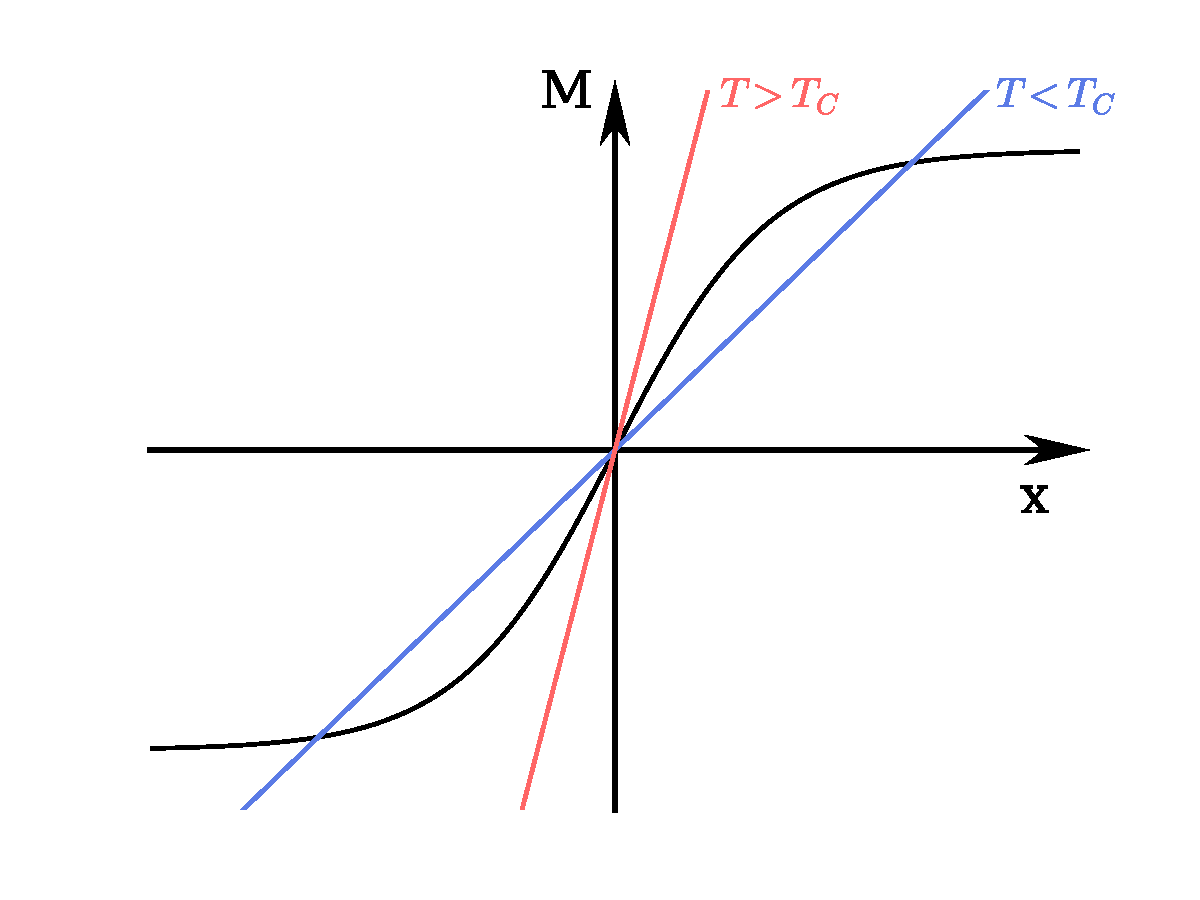
\includegraphics[width=0.916\linewidth]{../img/ferromag_graph_sol.pdf}
%   \captionsetup{width=6.9cm}
    \captionsetup{width=.95\linewidth}
    \captionof{figure}{Illustration of the grafical solution of \ref{eq:ferromag_graph_sol}. the straight lines refer to different values of of $T$.}
  \end{minipage}%
  \begin{minipage}[c][6.00cm]{.5\textwidth}
    \vspace*{\fill}
    \centering
    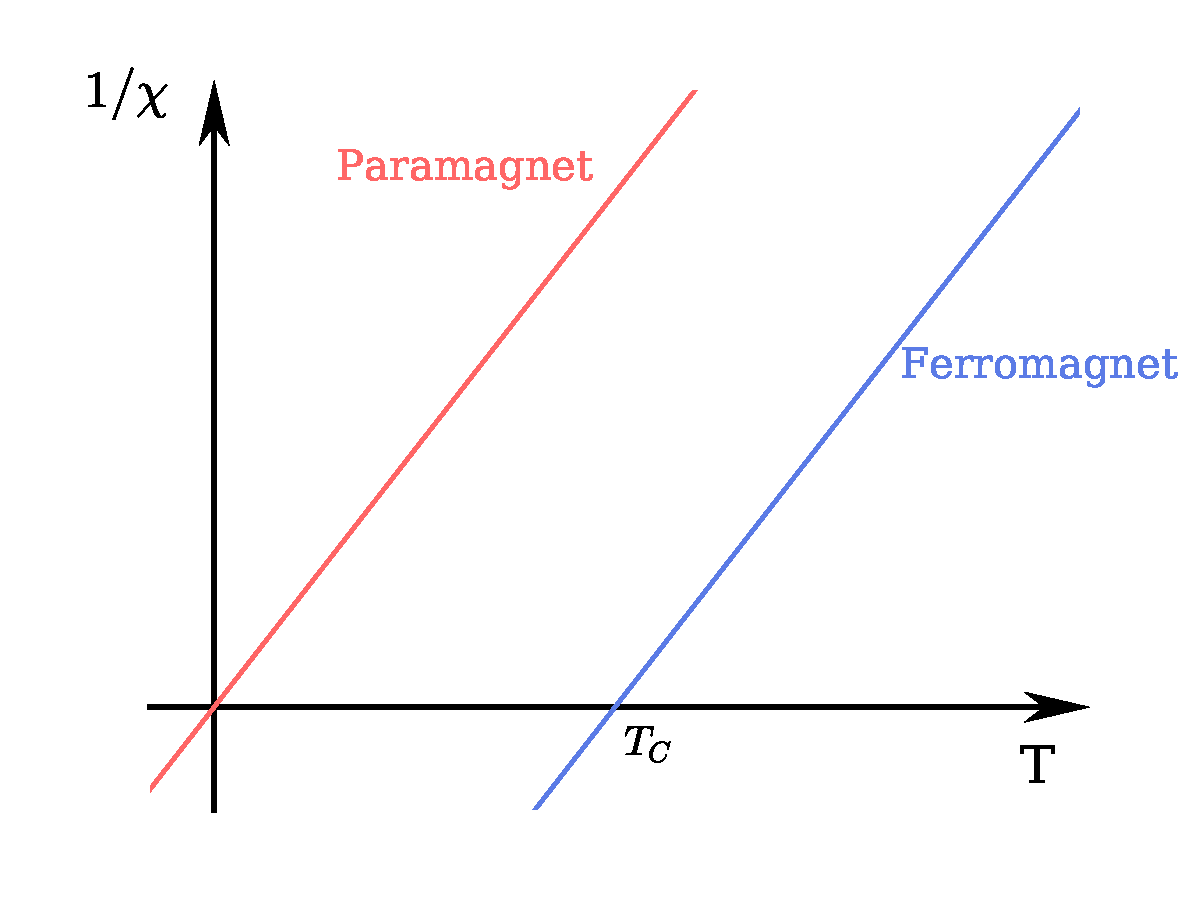
\includegraphics[width=0.95\linewidth]{../img/ferro_para_compar.pdf}
    \captionsetup{width=.95\linewidth}
 %   \captionsetup{width=6.9cm}
    \captionof{figure}{Illustration of susceptibility $\chi$ of a Para- and Ferromagnet.}
  \end{minipage}
  \label{fig:2:tests}
\end{figure}


%\begin{figure}
%  \centering
%  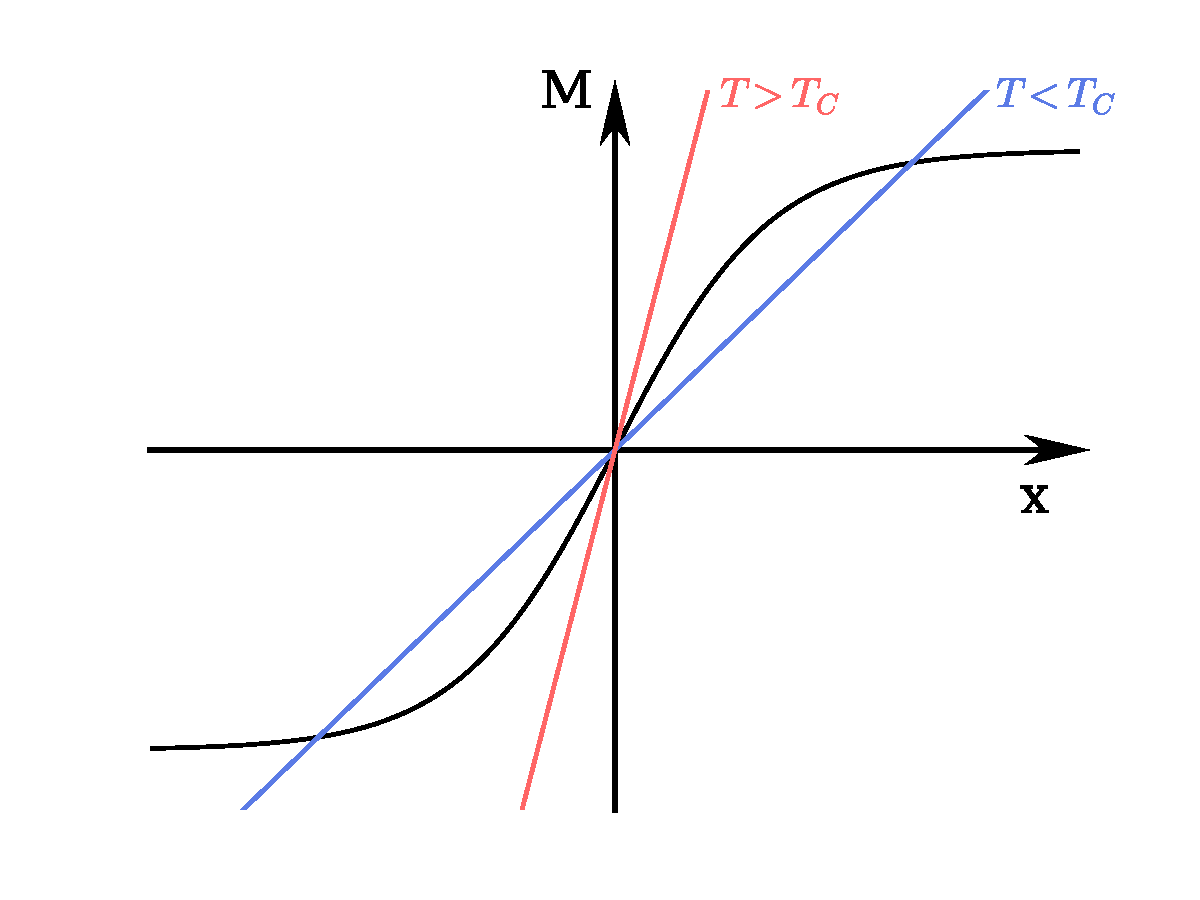
\includegraphics[width=0.5\linewidth]{../img/ferromag_graph_sol.pdf}
%  \caption{Illustration of the grafical solution of \ref{eq:ferromag_graph_sol}. the straight lines refer to different values of of $T$.}
%  \label{fig:ferromag_graph_sol}
%\end{figure}




Looking at the limit $ x \ll 1$ 

\begin{equation*}
  \left.
  \begin{array}{lcr}
    M ~ & = &~ C B/T \\
    \chi ~ & \equiv &~ M/B ~=~ C/T
  \end{array} \right\} 
  ~~~~ \rightarrow ~~~~ 
  \begin{array}{lcr}
    M ~~&=& ~ C \frac{B + \lambda M}{T}\\
    \chi ~ &\equiv& ~ \frac{C}{T} + \frac{\lambda}{T} \chi
  \end{array}
  ~~~~ \Rightarrow ~~~~ 
  \chi ~=~ \frac{C}{T-\lambda C} ~=~ \frac{C}{T - T_C}
\end{equation*}


Checking the magnetisation $M(T)$ at zero field $\vec{B} = 0$. Using \ref{eq:ferromag_graph_sol} with zero field and the definitinos $m = M/N \mu_B$ and $t = k_BT/N \mu_B^2 \lambda = T/T_C$ we get

\begin{equation}
  m ~~=~~ \tanh(\frac{m}{t})
\end{equation}

\begin{figure}[t]
  \begin{minipage}[c][6.00cm]{.5\textwidth}
    \vspace*{\fill}
    \centering
    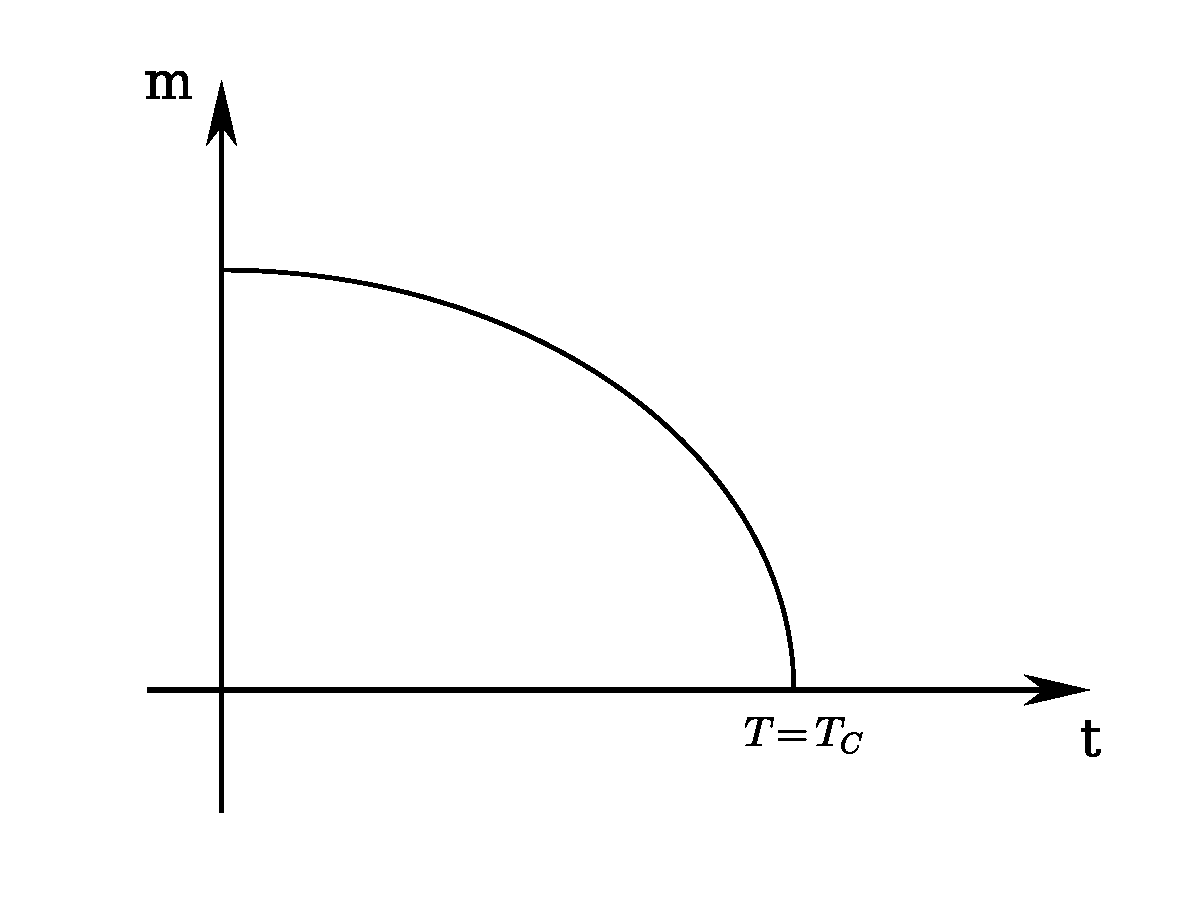
\includegraphics[width=0.916\linewidth]{../img/ferromag_M_T.pdf}
%   \captionsetup{width=6.9cm}
    \captionsetup{width=.95\linewidth}
    \captionof{figure}{Temperature dependence of magnetisation.}
  \end{minipage}%
  \begin{minipage}[c][6.00cm]{.5\textwidth}
    \vspace*{\fill}
    \centering
    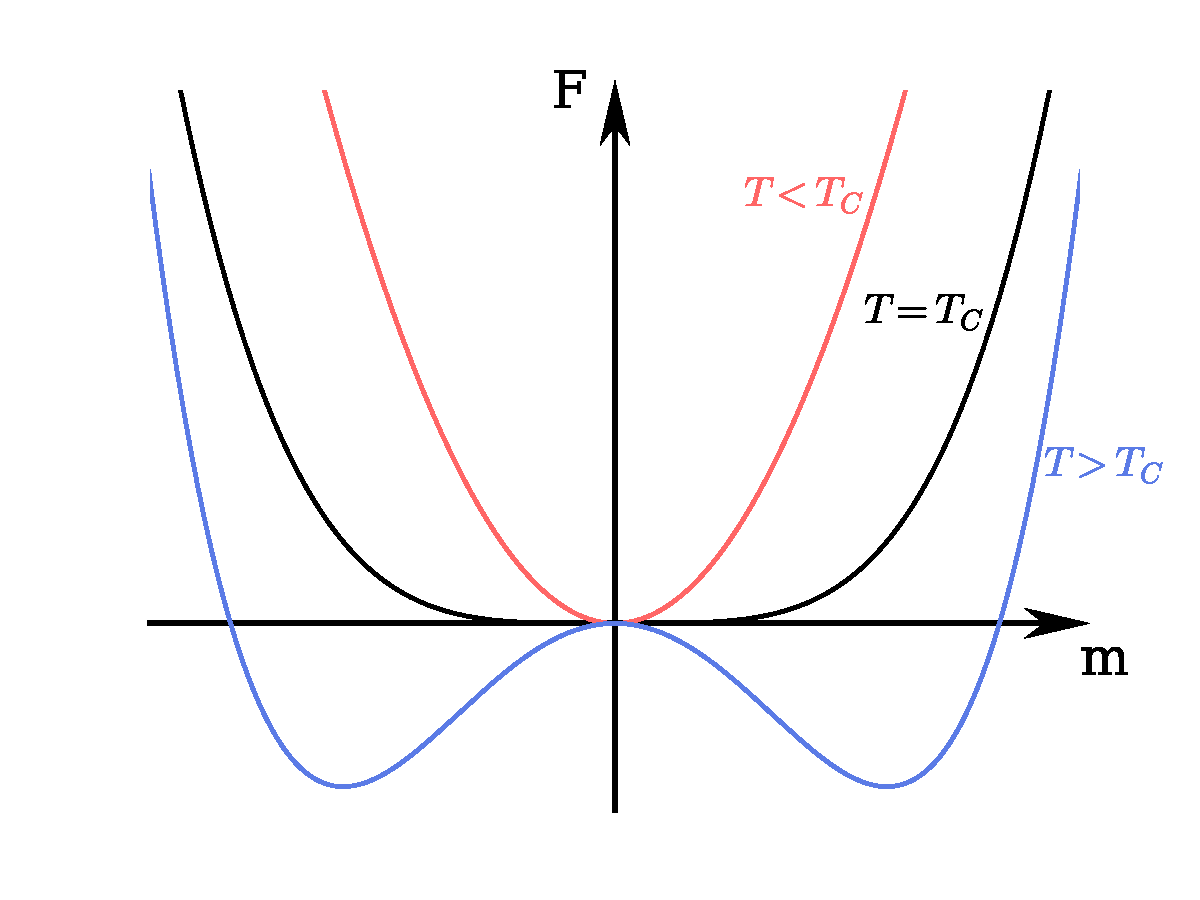
\includegraphics[width=0.95\linewidth]{../img/ferromag_landau.pdf}
    \captionsetup{width=.95\linewidth}
 %   \captionsetup{width=6.9cm}
    \captionof{figure}{Free Energy dependence on the order parameter $m$ for the 3 cases $T<T_C$, $T=T_C$ and $T>T_C$.}
  \end{minipage}
  \label{fig:2:tests}
\end{figure}


\subsubsection{Landau Theory}

According to the Landau theory of phase transisiton the free energy $F$ can be expressed

\begin{equation} \label{eq:ferromag_landau}
  F ~~=~~ F_0 ~+~ a(T) m^2 ~+~ b m^4 + ... 
\end{equation}

Were the parameter $a$ and $b$ has to meet the conditions

\begin{equation} \label{eq:ferromag_landau_condition}
  a(T) ~=~ a_0(T-T_C) ~~~~ \text{and} ~~~~ b>0
\end{equation}

We find the thermodynamical state of our system by minimizing the free energy

\begin{equation}
  \frac{dF}{dm} ~=~ m ( 2a(T) ~+~ 4bm^2) ~=~ 0 ~~~~ \Rightarrow ~~~~ m ~=~ \left\{ 
  \begin{array}{c}
    0\\
    \pm \sqrt{\frac{a_0(T-T_C)}{2b}}
  \end{array}
  \right.
\end{equation}



\subsection{Exchange Interaction J}


\begin{figure}
  \centering
  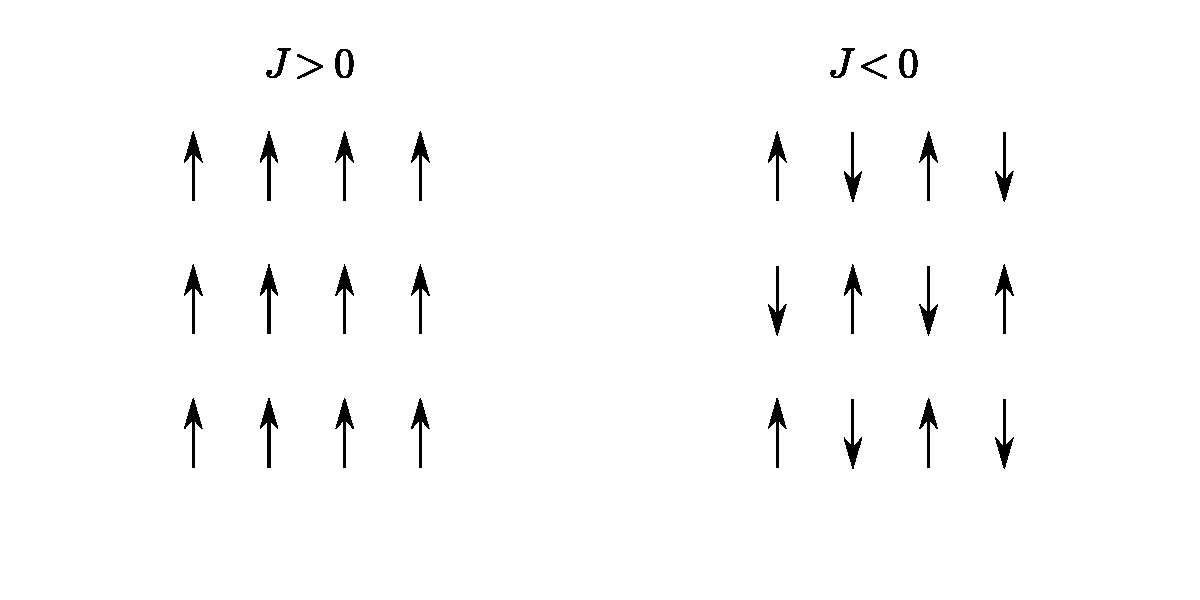
\includegraphics[width=0.7\linewidth]{../img/exch_spin_config.pdf}
  \caption{hohoho}
\end{figure}


Analog to the susceptibility of ferromagnets $\chi_{FM} = C/(T-T_C)$, we can define the susceptibility for anti-ferromagnets

\begin{equation}
  \chi_{AFM} ~~=~~ \frac{C}{T+T_N}
\end{equation}

Where we refer to the Transition Temperature $T_N$ as Neel-Temperature.


\begin{figure}[t]
  \begin{minipage}[c][6.00cm]{.5\textwidth}
    \vspace*{\fill}
    \centering
    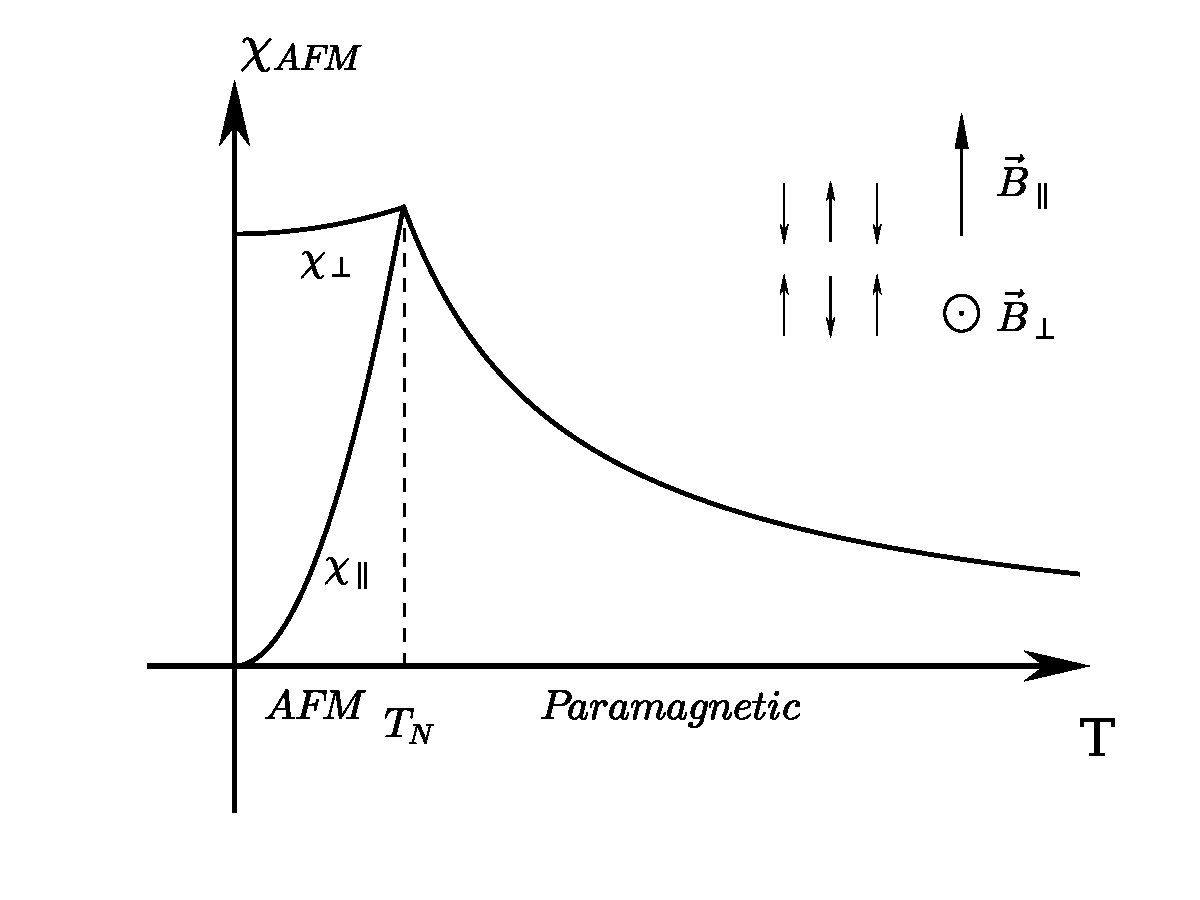
\includegraphics[width=0.916\linewidth]{../img/antiferro_suscept.pdf}
%   \captionsetup{width=6.9cm}
    \captionsetup{width=.95\linewidth}
    \captionof{figure}{Temperature dependence of magnetisation.}
  \end{minipage}%
  \begin{minipage}[c][6.00cm]{.5\textwidth}
    \vspace*{\fill}
    \centering
    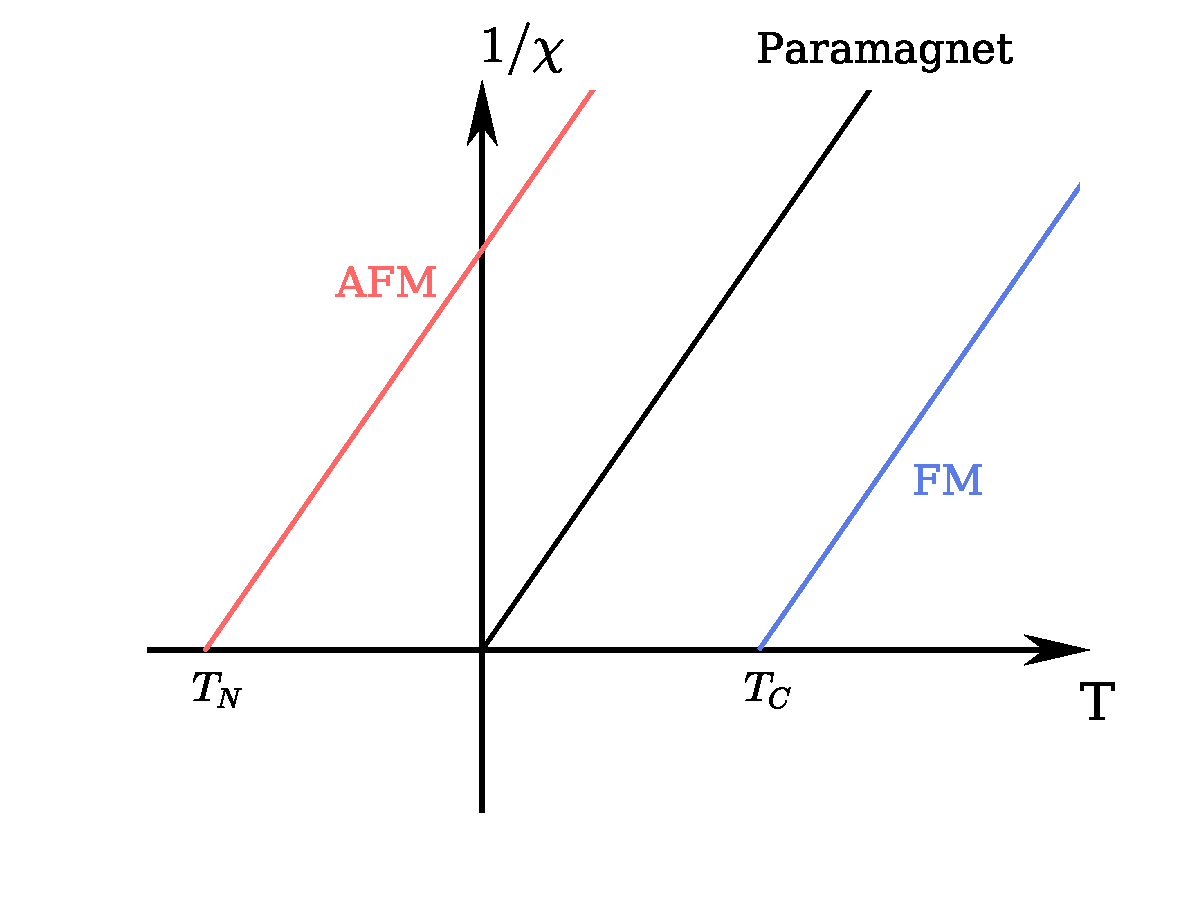
\includegraphics[width=1.0\linewidth]{../img/antiferro_para_compar.pdf}
    \captionsetup{width=1.0\linewidth}
 %   \captionsetup{width=6.9cm}
    \captionof{figure}{Free Energy dependence on the order parameter $m$ for the 3 cases $T<T_C$, $T=T_C$ and $T>T_C$.}
  \end{minipage}
  \label{fig:2:tests}
\end{figure}


\subsection{Ferromagnetic Magnons}

Consider a linear FM chain $ | \text{FM} \rangle ~=~ | \uparrow~ \uparrow~ \uparrow~ ...~ \rangle$. Applying the latter operator $ s^-_j$ onto this expression leads to

\begin{equation}
  | j \rangle ~~=~~ s^-_j | \text{FM} \rangle ~~=~~ 
  | \uparrow~ \uparrow~ ...~ \uparrow \underbrace{\downarrow}_{j} \uparrow~ ...~ \rangle
\end{equation}


Defining

\begin{equation}
  | q \rangle ~~=~~ \frac{1}{\sqrt{N}} \sum_j e^{i q R_j} | j \rangle
\end{equation}

The Hamilton is given as 

\begin{align}
  H ~~& =~~ - \sum_{ij} J_{ij} \hat{S}_i \cdot \hat{S}_j ~~=~~ -2J \sum_i \hat{S}_i \cdot \hat{S}_{i+1}\nonumber \\
      & =~~ - 2J \sum_i \left\{ \hat{S}^z_i \hat{S}^z_{i+1} ~+~ 
      \frac{1}{2} \left[ \hat{S}^+_i \hat{S}^-_{i+1} + \hat{S}^-_i \hat{S}^+_{i+1} \right]  \right\}
\end{align}

By taking only nearest neighbour interactions into account we get the 
The second equality sign holds if we only take neares neighbour interactions into account. To get the final expression we used the substitution

\begin{equation}
  \hat{S}^2 ~~=~~ \hat{S}^{z^2} ~+~ \frac{1}{2} \left[ \hat{S}^+_i \hat{S}^-_{i+1} + \hat{S}^-_i \hat{S}^+_{i+1} \right]
\end{equation}


\begin{equation}
  H | \text{FM} \rangle ~~=~~ -2 J N S^2 | \text{FM} \rangle ~~=~~ E_0 | \text{FM} \rangle
\end{equation}

\begin{equation}
  H | j \rangle ~~=~~ -2J \left\{ (N-4) S^2 | j \rangle ~+~ S \left[ |j+1\rangle + |j-1\rangle \right] \right\}
\end{equation}

\begin{align}
  H | q \rangle ~~& =~~ \frac{1}{\sqrt{N}} \sum_j e^{i q R_j} \left\{
  NS^2 |j\rangle ~-~ 2S^2|j\rangle ~+~ S |j+1\rangle ~+~ S|j-1\rangle \right\} \nonumber \\
                  & =~~ -2JNS^2 |q\rangle - 2J \left\{ -2S^2 ~+~ \left( e^{iqa} + e^{-iqa} \right) \right\} |q\rangle \nonumber \\
                  & =~~ E_0 |q\rangle ~+~ 2JS \left\{ 1 - \cos(qa) \right\} |q\rangle 
\end{align}

%%%% one equation not transcripted from lecture notes %%%


Since we are consindering an infinit long 1D chain of spin states we can rewrite the expression

\begin{equation}
  H |q\rangle ~~=~~ E_0 |q\rangle + 2JS \left\{ 2 - 2\cos(qa) \right\} |q\rangle
\end{equation} 

which leads to

\begin{equation}
  H |q\rangle ~~=~~ E(q) |q\rangle ~~~~~ \text{with} ~~~~ E(q) ~≃~ E_0 + 2JS(2 - 2\cos(qa))
\end{equation}

This is the dispersion relation for ferromagnets. For anti-ferromagnets we have a similar relation (not derived)

\begin{equation}
  \hbar \omega ~~=~~ 2J | \sin(qa) |
\end{equation}


%===============================================================================================================
% Superconductivity
%===============================================================================================================

\chapter{Superconductivity}

\section{Conventional superconducters}

\subsection{Link $\rho$ \& Meissner Effect}

\begin{figure}
  \centering
  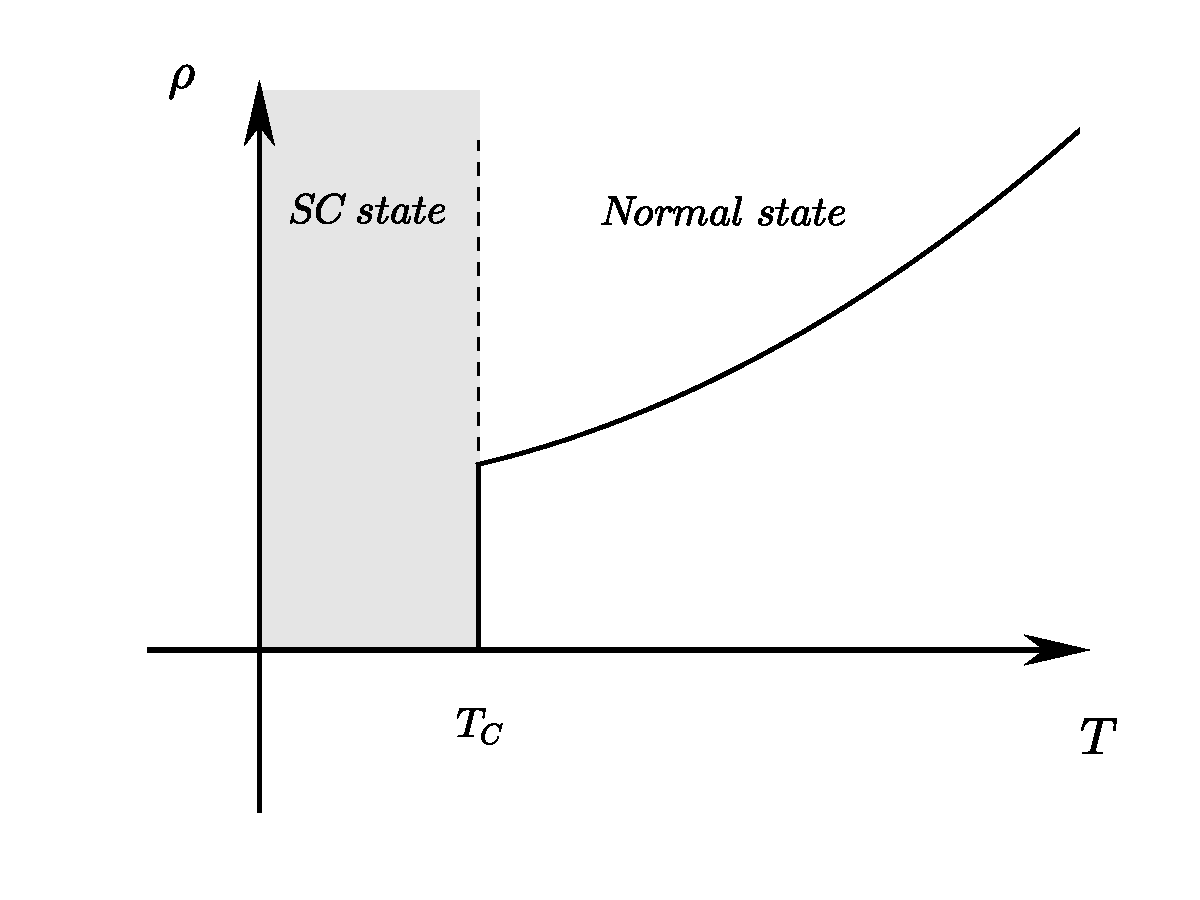
\includegraphics[width=0.7\linewidth]{../img/sc_resistivity_drop.pdf}
  \caption{hohoho}
  \label{fig:sc_res_drop}
\end{figure}


As we know, superconductors are characterised by vanishing resistvity ($\rho=0$) for undergoing a critical temperature $T_C$ (\myRef{fig:sc_res_drop}).
Recalling Ohm's law, 

\begin{equation} \label{eq:ohms_law}
  \vec{j} ~~=~~ \sigma \vec{E}
\end{equation}


which relates the electron current density $\vec{j}$ and the electric field inside a conductor $\vec{E}$ by introductin the material dependent conductivity $\sigma$.

Looking at the case of superconductors, we can emphasize, by rearranging Ohm's law, that the electric field vanishes.

\begin{equation}
  \vec{E} ~~=~~ \frac{1}{\sigma} \vec{j} ~~=~~ \rho \vec{j} ~~≃~~ 0
\end{equation}

By using one of the Maxwell equation $\nabla \times \vec{E} = - d\vec{B}/ dt$ we can conclude, that for a vanishing electric field $\vec{E} = 0$ there can't be a change of the magnetic field over time $d\vec{B}/dt=0$.


\textcolor{red}{diagram vanishing B-field}


\subsection{London Equation}

The lonodon equation is a macroscopic theory that was one of the first theories which allowed to describe effects like the Meissner-Ochsenfeld effect quantitatively.
We know want to qualitiatively derive the london equation. For that consider a current oscillating if the frequency $\omega$

\begin{equation}\label{eq:osc_curr}
  \vec{j} e^{-i \omega t} ~~=~~ \sigma(\omega) \vec{E} e^{-i \omega t}
\end{equation}

Using the expression for the conductivity $\sigma(\omega)$ from the Drude model for a time-dependent electric field

\begin{equation}
  \sigma(\omega) ~~=~~ \frac{\vec{j}}{\vec{E}} ~~=~~ \frac{ne^2 \tau}{m} \frac{1}{1-i\omega \tau}
\end{equation}

%Looking at the real part of the conductivity
%
%\begin{equation}
%  \Re(\sigma(\omega)) ~~=~~ \frac{ne^2}{m} \frac{\tau}{1+\omega \tau}~~ \xrightarrow{\omega \rightarrow 0} ~~
%  \frac{ne^2 \tau}{m}
%\end{equation}

From this we get, as already proven in a previous excercise, that the real part of the conductivity can be written in the limit of $\tau \rightarrow \infty$ as

\begin{equation}\label{eq:real_conduct}
  \Re(\sigma(\omega)) ~~=~~ \frac{\pi n e^2}{m} \delta(\omega)
\end{equation}


This can also be made clear, when looking at the limits

\begin{equation}
  \Re(\sigma(\omega)) ~~=~~ \frac{ne^2}{m} \frac{\tau}{1+\omega \tau}~~ \xrightarrow{\omega \rightarrow 0} ~~
  \frac{ne^2 \tau}{m}
\end{equation}

\begin{equation}
  \sigma(\omega) ~~ \xrightarrow{\tau \rightarrow \infty} ~~ -\frac{ne^2}{im\omega} = \Im(\sigma(\omega)) ~~~~ \Rightarrow ~~~~ \Re(\sigma(\omega)) = 0 ~~~~~~\text{for}\ \omega \neq 0
\end{equation}


From \myEq{eq:real_conduct}, we see that in the regime of very large mean free times $\tau$ between ionic collisions, the real part of the conductivity $\sigma(\omega)$ is only different from zero for vanishing oscillations of the electric field. 

To derive the London equation, the following two assumptions have to be made

\begin{enumerate}
\item{$\tau \rightarrow \infty$, which is given since there are no collisions between electrons and lattice ions in the superconducting state.}
\item{We have to split up the conductivity in a part $\sigma_{N}(\omega)$ of normal state electrons and a conductivity contribution due to \textit{super electrons} $\sigma_{S}$: 
$\sigma(\omega) = \sigma_N(\omega) + \sigma_S(\omega)$, were only $\sigma_S(\omega) \neq 0$ in the superconducting state}
\end{enumerate}


Taking the curl of the oscillating current

\begin{align}\label{eq:curl_curr}
  \nabla \times (\vec{j} e^{-i\omega t}) & ~~=~~ -\sigma(\omega) \nabla \times (\vec{E}\cdot e^{-i\omega t}) ~~=~~
  -\sigma(\omega) \frac{d}{dt} (\vec{B} \cdot e^{-i\omega t})\nonumber \\
    & ~~=~~ - \frac{n_Se^2}{m} \vec{B} \cdot e^{-i\omega t}
\end{align}

Here we used \myEq{eq:osc_curr} in the first and farradays law ($\nabla \times \vec{E} = d/dt \vec{B}$) in the second step. Furthermore is only the \textit{super electron} density $n_S$ contributing to the conductivity $\sigma(\omega)$. From this equation we can deduce that

\begin{equation}\label{eq:london_eq}
  \nabla \times \vec{j} ~~\propto~~ \vec{B} ~~~~~~\text{and thereof}~~~~ \vec{j} = -\frac{n_Se^2}{m} \vec{A}
\end{equation}

with $\vec{A}$ being the vector potential. The equation describing this proprtionality between the current density $\vec{j}$ and the vector potential $\vec{A}$ is the London equation.


%The london equation allows us now to set up a differential equation for the magnetic field $\vec{B}$. 
%
Together with Ampere's law ($\nabla \times \vec{B} = \mu_0 \vec{j}$) allows us the London equation (\myEq{eq:london_eq}) now to set up a differential equation for the magentic field $\vec{B}$.

\begin{equation} \label{eq:deq_B_0}
  \nabla \times \nabla \times \vec{B} ~~=~~ -\frac{1}{\lambda^2} \vec{B}, ~~~~~~ \text{where}~~ 
  \lambda = \sqrt{\frac{m}{\mu_0 n_S e^2}}
\end{equation}

This equation can also be written as

\begin{equation} \label{eq:deq_B}
  \nabla^2 \cdot \vec{B} ~~=~~ \frac{1}{\lambda^2} \vec{B}
\end{equation}


To exemplify the solution of this differential equation we look at it in one dimension. Then \myEq{eq:deq_B} becomes $d^2/dx^2 B_z(x) = 1/\lambda^2 B_x$.

To exemplify the solution of this differential equation we look at a situation were we have a superconductor filling the space for all values $x\geq 0$ correspinding to that we have vacuum at $x<0$. Applyling now a magnetic field in the vacuum region aligned along the z-axis $\vec{B} = (0,0,B_0)$. in this case the differential equation \myEq{eq:deq_B} simplifies to 

\begin{equation}
  \frac{d^2}{dx^2} B_z(x) ~~=~~ \frac{1}{\lambda^2} B_z(x)
\end{equation}

Using the boundary conditions $B_z(x) \xrightarrow{x \rightarrow \infty} 0$ (Meissner Effect) and $B_z(x \rightarrow 0)=B_0$ leads to the solution

\begin{equation} \label{eq:B_decrease}
  B_z(x) ~~=~~ B_0 e^{-x/\lambda}
\end{equation}

This solution describes an exponentially decreasing magnetic field inside the the superconductor close to the surface. From this formula one can also recognize that $\lambda = \sqrt{m/\mu_0 n_S e^2}$ introduced a characteristic length scale over which the magnetic penetrates the superconductor. For that reason $\lambda$ is referred to as \textit{London penetration depth}. 
In \ref{fig:london_lambda} we see \myEq{eq:B_decrease} plotted for two different values of lambda $\lambda_1 > \lambda_2$. 
Looking at the definition of the London penetration depth we see that $n_{S_1} < n_{S_2}$, which means that the higher the charge density the more is the penetrating magnetic field $B_z(x)$ diminished.


\begin{figure}[t]
  \begin{minipage}[c][6.00cm]{.5\textwidth}
    \vspace*{\fill}
    \centering
    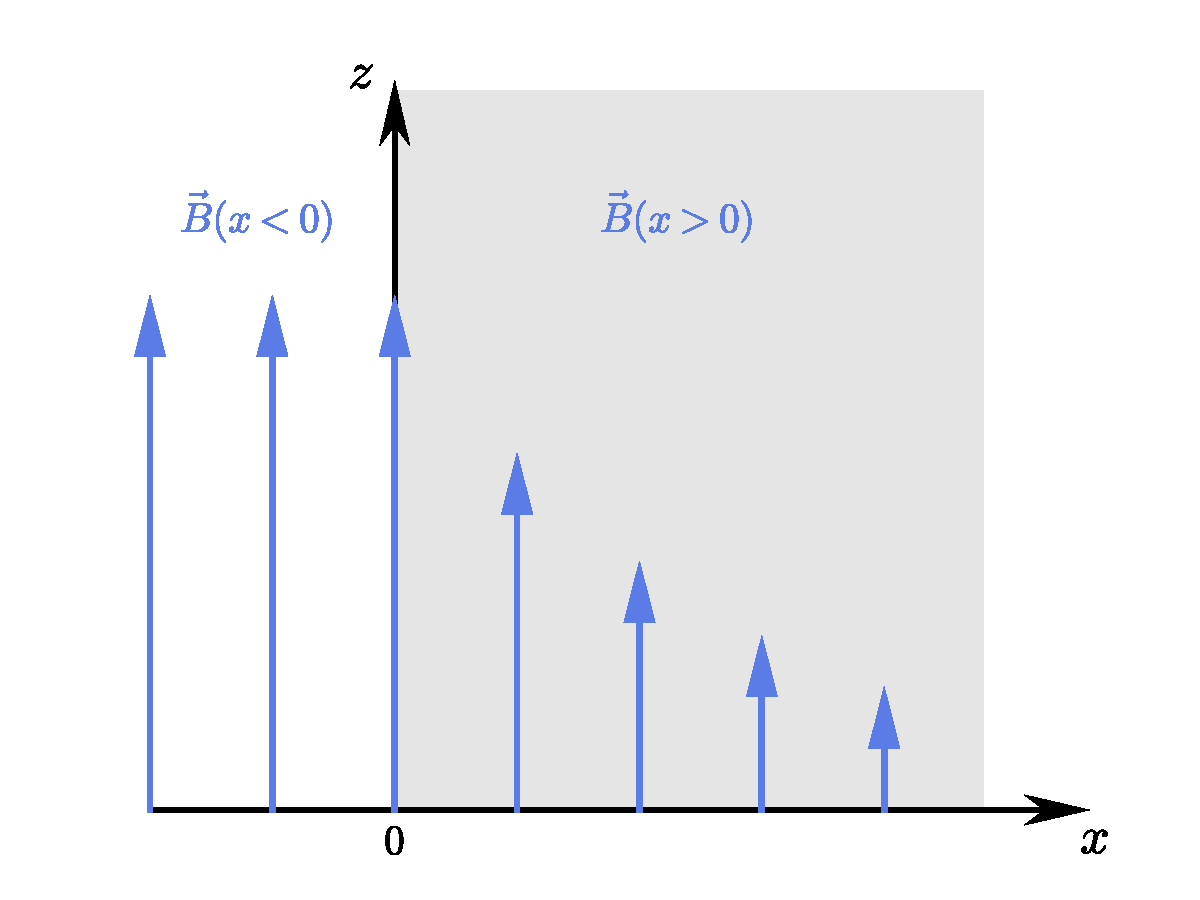
\includegraphics[width=0.916\linewidth]{../img/london_B_1dim.pdf}
%   \captionsetup{width=6.9cm}
    \captionsetup{width=.95\linewidth}
    \captionof{figure}{Illustration of the magnetic field decrease inside the superconductor according to \myEq{eq:B_decrease}. The magnetic field is pictorially drawn as blue vectors. Adapted from \text{red}{Kittel - include citation}}
    \label{fig:london_B_1dim}
  \end{minipage}%
  \begin{minipage}[c][6.00cm]{.5\textwidth}
    \vspace*{\fill}
    \centering
    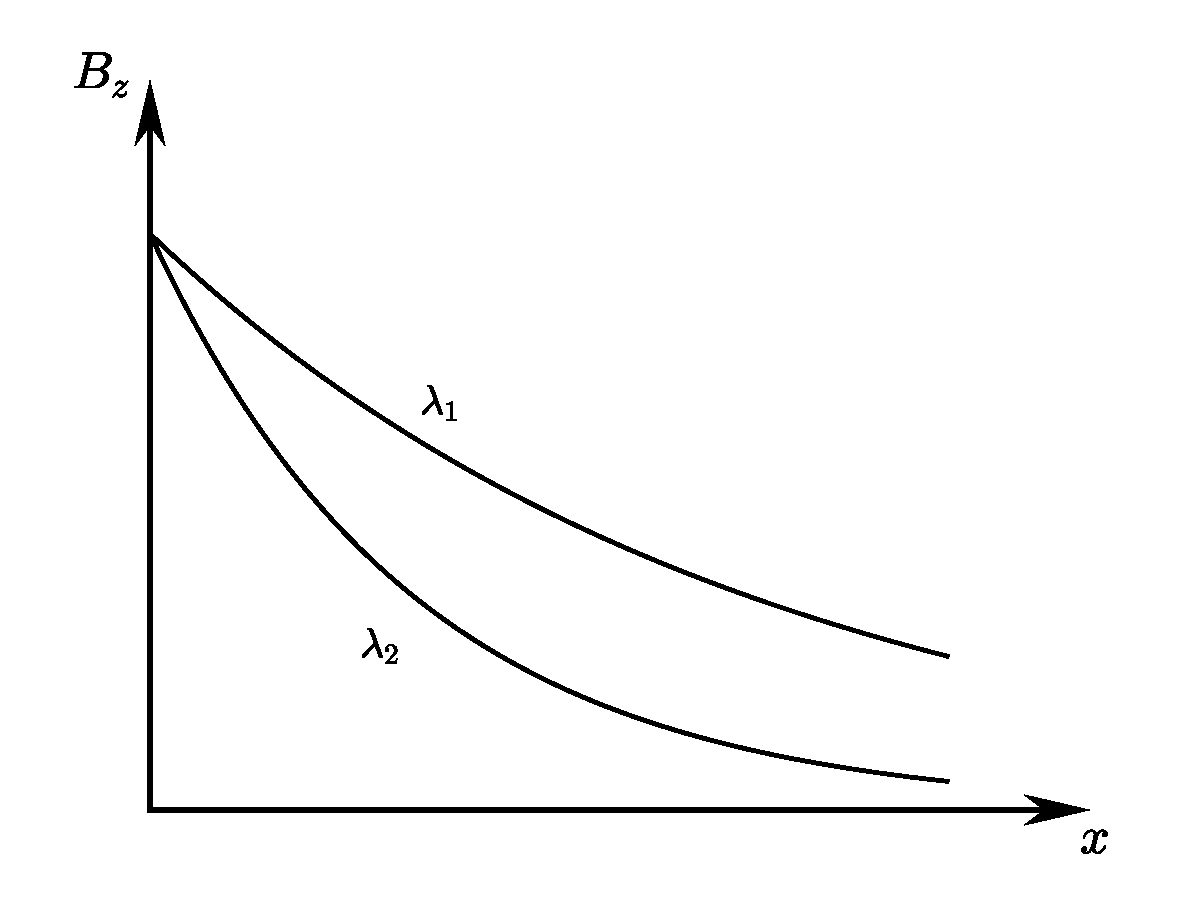
\includegraphics[width=1.0\linewidth]{../img/london_lambda.pdf}
    \captionsetup{width=0.95\linewidth}
 %   \captionsetup{width=6.9cm}
    \captionof{figure}{Illustration of \myEq{eq:B_decrease} for two different values for the london penetration depth.}
    \label{fig:london_lambda}
  \end{minipage}
\end{figure}




\subsection{Coherence Length}

Another lengthscale that helps us to classify the different types of superconductors is the \textit{coherence length} $\xi$. The coherence length is a measure of the distance within which the superconducting electron concentration cannot change drastically in a spatially-varying magnetic field.

\begin{equation} \label{eq:coherence_length}
  \xi ~~=~~ \frac{\hbar v_F}{\pi \Delta}
\end{equation}

Where $v_F$ stands for the fermi velocity and $\Delta$ for superconducting gap being present at the fermi surface in the SC state. $\xi$ is a parameter in the \textit{Ginzburg-Landau Theory} and can be derived there.

The two length scales, penetration depth and coherence length, allow us now, to categorize the superconductors in the groups \textit{Type 1} and \textit{Type 2}. This goes as follows:

By defining $\kappa \equiv \xi/\lambda$ we say a Superconductor contains to the group of \textit{Type 1} (\textit{Type 2}) if $\kappa ~<~ (>)~ 1/\sqrt{2} \simeq 0.707 $. 

Values of $\kappa$ for some materials are given in \textcolor{red}{lenght scale table}. The classification of SC into Type 1 and Type 2 does not fully coincide with the classification of conventional and unconvential. Although a lot of the conventional (elementary) supperconductors are of Type 1, there are also some expetions like Niobium (Nb) which is a conventional Type 2 Superconductor.

\textcolor{red}{include table from PPP}


\subsection{Ginzburg-Landau Theory}

The Landau Theory of Phase Transtition can also be used in the case of the transition from normal to superconducting state. The free energy per volume of the system in the superconducting state is given as

\begin{equation}
  f_\text{SC} ~~=~~ f_\text{NS} ~+~ a(T) |\psi(T)|^2 ~+~ \frac{1}{2} b(T) |\psi(T)|^4 ~+~ ...
\end{equation}

$|\psi|$ is treated as the order parameter. 
To find the temperature dependence of the free energy per volumne we make the following assumptions: near the transition temperature $T_C$ has $a$ to be linear in temperature ($a(T)=a_0(T-T_C) +...$) and $b$ given as $b(T)=b_0+...$ with $a_0, b_0$ being constant and larger than zero.

Looking for the extrema of $(f_\text{SC}-f_\text{NS})$

\begin{equation} \label{eq:f_SC_derived}
  \frac{d (f_\text{SC}-f_\text{NS})}{d|\psi|} ~~=~~ 2|\psi| \left\{a(T) ~+~ b(T)|\psi|^2  \right\} 
  ~~\overset{!}{=}~~ 0
\end{equation}

We find the following condition for $|\psi|$ to minimize $(f_\text{SC}-f_\text{NS})$

\begin{equation} \label{eq:psi_condition}
  |\psi| ~~=~~ \left\{ 
  \begin{array}{cr}
    0, & T>T_C\\
    \pm \sqrt{-a(T)/b(T)}, & T<T_C
  \end{array} \right.
\end{equation}

Plugging \myEq{eq:psi_condition} into \myEq{eq:f_SC_derived} leads to

\begin{equation}
  (f_\text{SC} - f_\text{NS}) ~~=~~ -\frac{a^2(T)}{b(T)} ~+~ \frac{1}{2} \frac{a^2(T)}{b(T)} ~~=~~
  -\frac{1}{2} \frac{a_0^2(T-T_C)^2}{b_0}
\end{equation}


\begin{figure}[t]
  \begin{minipage}[c][6.50cm]{.5\textwidth}
    \vspace*{\fill}
    \centering
    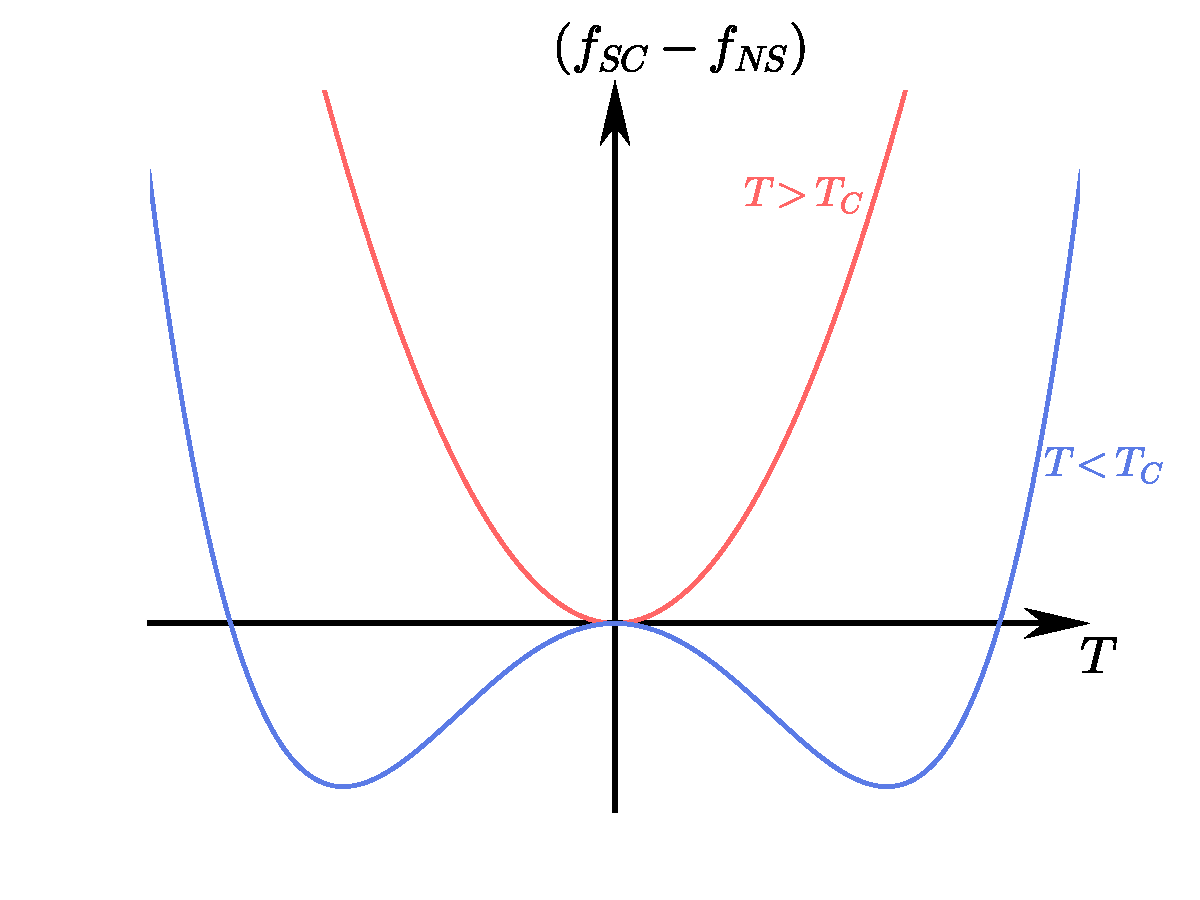
\includegraphics[width=0.916\linewidth]{../img/landauginzburg_f_SC.pdf}
%   \captionsetup{width=6.9cm}
    \captionsetup{width=.95\linewidth}
    \captionof{figure}{Difference of the free energy per volume between the normal- and superconducting state.}
    \label{fig:london_B_1dim}
  \end{minipage}%
  \begin{minipage}[c][6.00cm]{.5\textwidth}
    \vspace*{\fill}
    \centering
    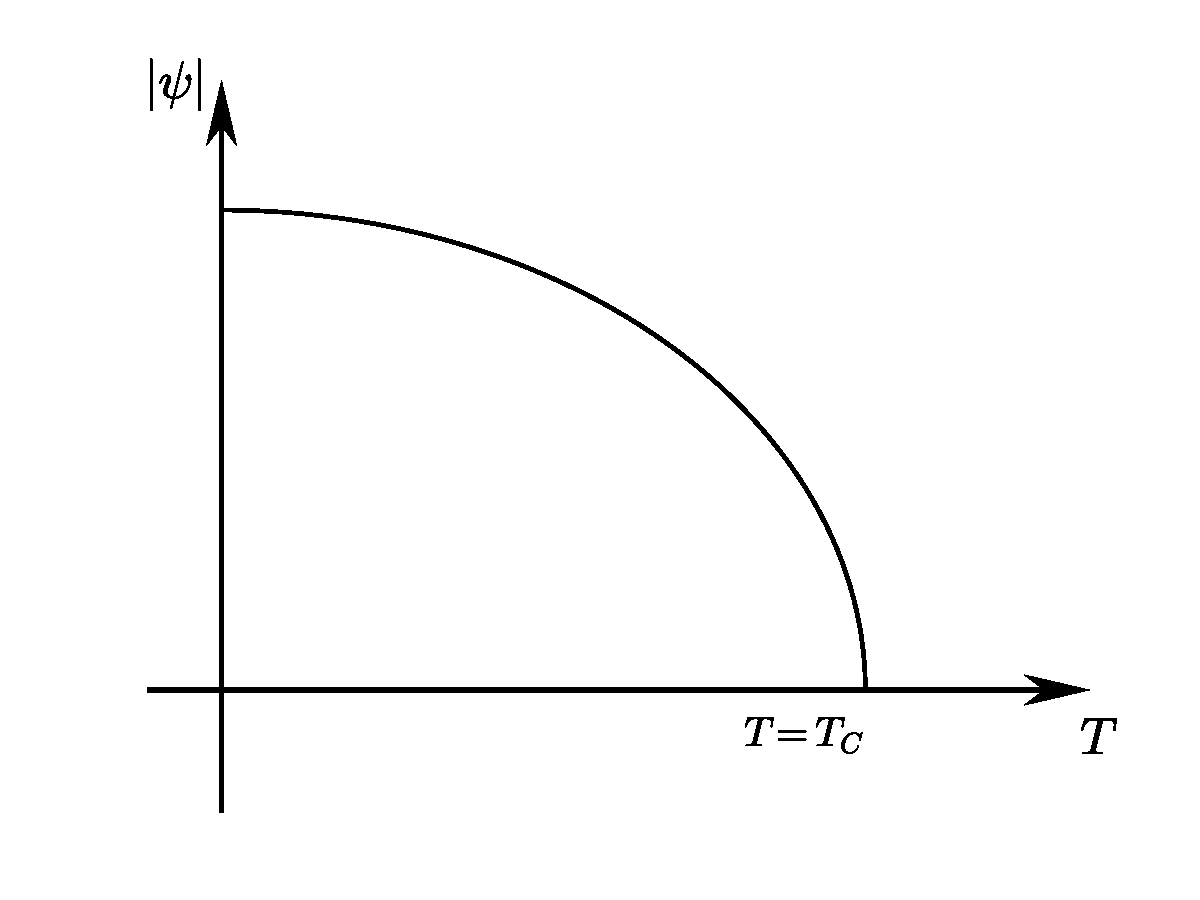
\includegraphics[width=1.0\linewidth]{../img/landauginzburg_psi_T.pdf}
    \captionsetup{width=0.95\linewidth}
 %   \captionsetup{width=6.9cm}
    \captionof{figure}{Temperature dependence of the order parameter $|\psi|$. }
    \label{fig:london_lambda}
  \end{minipage}
\end{figure}

Since $f_\text{SC}$ is the free energy, we can write

\begin{equation}
  S ~~\equiv~~ -\frac{df}{dT} ~~~~~~\text{and}~~~~~~ C ~~\equiv~~ T \cdot \frac{dS}{dT}
\end{equation}

This gives for the difference in the heat capacity

\begin{equation} \label{eq:diff_heat_cap}
  \Delta C ~~\equiv~~ C_\text{SC} ~-~ C_\text{NS} ~~=~~ -T \frac{d^2(f_\text{SC}-f_\text{NS})}{dT^2} 
  ~~=~~ T \frac{a_0^2}{b_0}
\end{equation}

Evaluating \myEq{eq:diff_heat_cap} at the transition Temperature gives us the jump in specific heat at the phase transition

\begin{equation}
  \Delta C(T_C) ~~=~~ \frac{a_0^2}{b_0} T_C
\end{equation}


\subsection{Classification of different superconductors}


\subsection{Vorteces}

To define the appearance of vorteces from Type 2 Superconductors into into our formalism we define the free energy per volumne as

\begin{equation} \label{eq:vortex_free_energy}
  f_\text{SC} - f_\text{NS} ~~≃~~ a(T) |\psi(r)|^2 ~+~ b(T)|\psi(r)|^4 ~+~ 
  \frac{\hbar^2}{2m} \nabla |\psi|^2
\end{equation}

To get the total Free energy we integrate \myEq{eq:vortex_free_energy} over all space

\begin{equation}
  F_\text{SC} - F_\text{NS} ~~=~~ \int d^3r (f_\text{SC} - f_\text{NS})
\end{equation}

We are interested now in finding the wavefunction $\psi(r)$ for which the Free energy is minimized. Since $\psi(r)$ is a function, this condition is formulated in a functional of the following form

\begin{equation}
  \frac{\delta F_\text{SC}}{\delta \psi(r)} ~~\overset{!}{=}~~ 0
\end{equation}

This is a differential equation for $\psi(r)$. In one dimnesion this DEG looks like the following

\begin{equation} \label{eq:vortex_wave_function_deg}
  -\frac{\hbar^2}{2m} \frac{d^2\psi(x)}{dx^2} ~+~ a(T) \psi(x) ~+~ b(T) \psi^3(x) ~~=~~ 0
\end{equation}

A solution to this differential equation is

\begin{equation} \label{eq:vortex_wave_function}
  \psi(x) ~~=~~ \psi_0 \tanh(\frac{x}{\sqrt{2} \xi(T)})
  \ 
\end{equation}


The coherence length $\xi(T)$ introduces a temperature dependent length scale and is given as

\begin{equation} \label{eq:vortex_coherence_length}
  \xi(T) ~~=~~ \left( \frac{\hbar}{2m |a(T)|} \right)^{1/2} ~~=~~ \xi_0\ t^{-1/2} ~~~~~~\text{with}~~~~ 
  t = \frac{T-T_C}{T_C}
\end{equation}

Here we used the same expression for $a(T)$ as in the ginzburg-Landau Theory.

\begin{figure}[t]
  \begin{minipage}[c][6.50cm]{.5\textwidth}
    \vspace*{\fill}
    \centering
    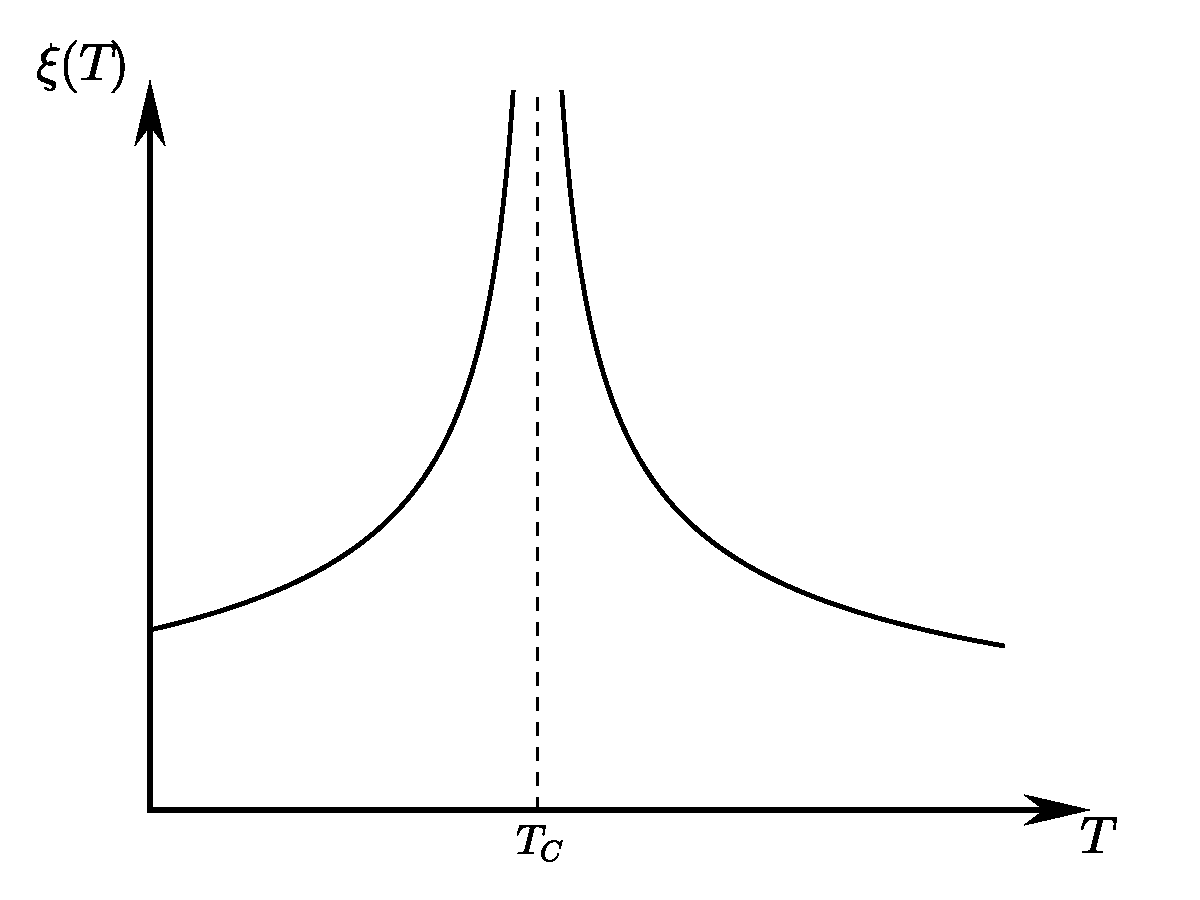
\includegraphics[width=0.916\linewidth]{../img/vortex_coherence_length.pdf}
%   \captionsetup{width=6.9cm}
    \captionsetup{width=.95\linewidth}
    \captionof{figure}{Coherence length $\xi(T)$ plotted over Temperature according to \myEq{eq:cortex_coherence_length}. Noteworthy is the diverging of $\xi$ when going close to $T_C$.}
    \label{fig:london_B_1dim}
  \end{minipage}%
  \begin{minipage}[c][6.00cm]{.5\textwidth}
    \vspace*{\fill}
    \centering
    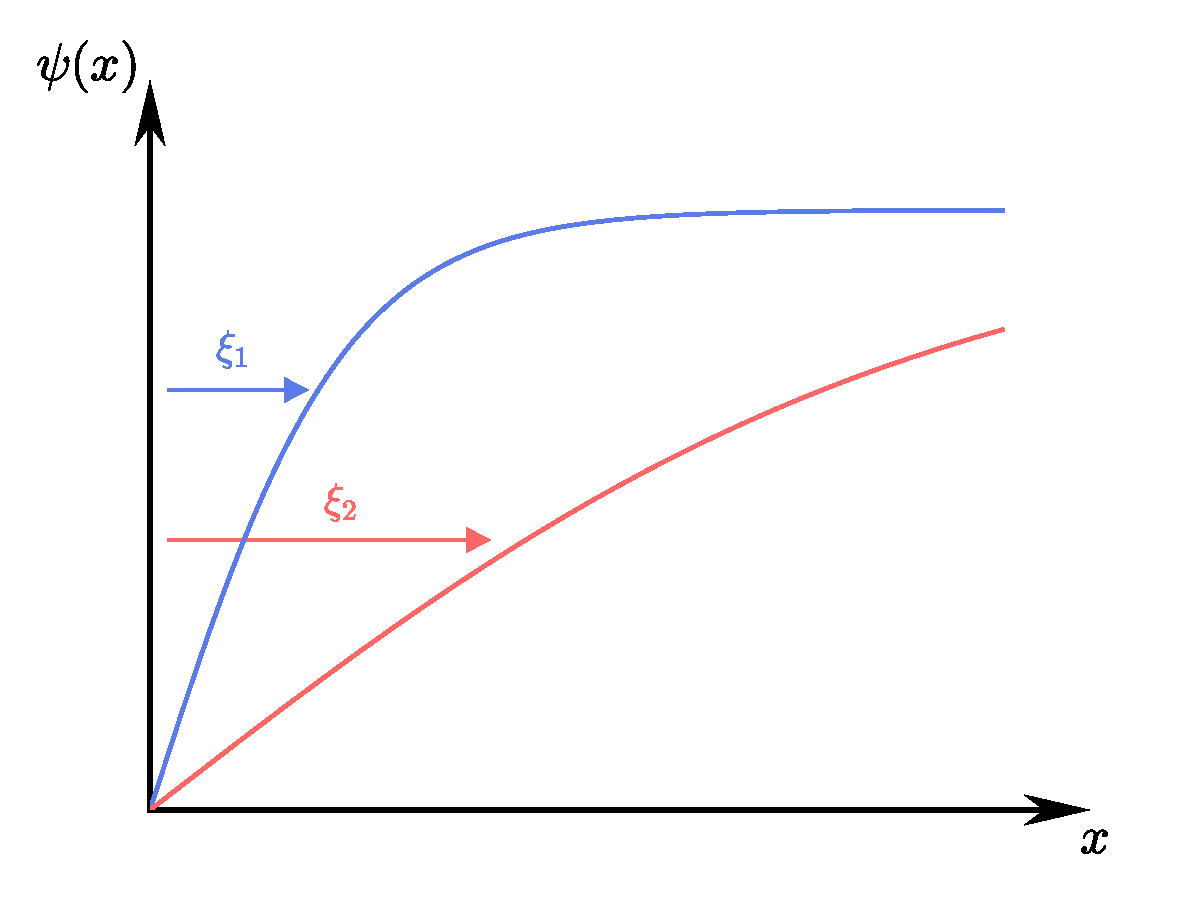
\includegraphics[width=1.0\linewidth]{../img/vortex_wavefunction.pdf}
    \captionsetup{width=0.95\linewidth}
 %   \captionsetup{width=6.9cm}
    \captionof{figure}{Wavefunction in one dimension according to \myEq{eq:vortex_wave_function}. Comparing the the blue and red curve shows that the wave function gets \textit{pushed down} for increasing coherence length ($\xi_2 > \xi_1$).}
    \label{fig:london_lambda}
  \end{minipage}
\end{figure}




%========================================================================================================
%========================================================================================================
%========================================================================================================


\begin{thebibliography}{9}

%\bibitem{bednorz86}
%  J.G. Bednorz and K.A. Müller,
%  Possible High T\textsubscript{c} Superconductivity in the Ba-La-Cu-O System
%  \textit{Condens. Matter}, \textbf{64}:189-,
%  1986.
%
%\bibitem{schilling93}
%  A. Schilling, M. Cantoni, J.D. Guo and H.R. Ott,
%  Superconductivity above 130 K in the Hg-Ba-Ca-Cu-O system
%  \textit{Nature}, \textbf{363}:56-,
%  1993.
%  
%\bibitem{ray15}
%  Pia J. Ray,
%  \textit{Master Thesis: Structural investigation of La\textsubscript{2-x}Sr\textsubscript{x}CuO\textsubscript{4}},
%  University of Copenhagen,
%  2015.
%
%
%
%\bibitem{lee06}
%  P. A. Lee, \textit{et. al},
%  Doping a Mott Insulator: Physics of high-temperature superconductivity,
%  \textit{Rev. Mod. Phys.}, \textbf{78}:17-,
%  2006.
%
%\bibitem{tokura00}
%  Y. Tokura, N. Nagaosa,
%  Orbital Physics in Transition-Metal Oxides,    
%  \textit{Science}, \textbf{288}:462-468,
%  2000.
%
%\bibitem{pickett89}
%  W. E. Pickett,
%  Electronic structure of the high-temperature oxid superconductors
%  \textit{Rev. Mod. Phys.}, \textbf{61}:433-,
%  1989.
%  
%\bibitem{emery87}
%  V. J. Emery,
%  Theory of High-$T_c$ Superconductivity in Oxides,
%  \textit{Phys. Rev. Lett.}, \textbf{58}:2794-,
%  1987.
%  
%\bibitem{zhang88}
%  F. C. Zhang and T. M. Rice,
%  Effective Hamiltonian for the superconducting Cu oxides,
%  \textit{Phys. Rev. B}, \textbf{37}:3759-,
%  1988.
%
%\bibitem{tanaka06}
%  S. Tanaka,
%  High-Temperature Superconductivity,
%  \textit{Jpn. J. Appl. Phys.}, \textbf{Vol.45, No.12}:9011-9024,
%  2006.
%  
%\bibitem{rhaman15}
%  Md. A. Rhaman \textit{et al.},
%  A Review on Cuprate Based Superconducting Materials Including Characteristics and Applications,
%  \textit{American Journal of Physics and Applications}, \textbf{Vol.3, No.2}:39-56,
%  2015.
%
%\bibitem{jahn37}
%  H. A. Jahn and E. Teller,
%  Stability of Polyatomic Molecules in Degenerate Electronic States,
%  \textit{Proc. R. Soc. London, Ser. A}, \textbf{161}:200-,
%  1937.
%
%\bibitem{damascelli03}
%  A. Damascelli \textit{et. al},
%  Angle-resolved photoemission studies on the cuprate superconductors,
%  \textit{Rev. Mod. Phys.}, \textbf{75}:473-,
%  2003.
%
%
%\bibitem{damascelli04}
%  A. Damascelli,
%  Probing the Electronic Structure of Complex Systems by ARPES,
%  \textit{Physica Scripta}, \textbf{T109}:61-,
%  2004.
%  
%\bibitem{hufner95}
%  S. H\"ufner,
%  Photoelectron Spectroscopy, 2nd Edition,
%  \textit{Springer-Verlag} New York,
%  1995.
%
%\bibitem{nolting7-7}
%  W. Nolting,
%  Viel-Teilchen-Theorie, 7th Edition,
%  \textit{Springer-Verlag} Berlin Heidelberg,
%  2009.
%
%\bibitem{wang12}
%  W.-P. Wang, \textit{et. al},
%  Orbital characters determined from Fermi surface intensity patterns using angle-resolved photoemission spectroscopy,
%  \textit{Physical Review B}, \textbf{85}:214518,
%  2012.
%
%\bibitem{osterwalder_pes}
%  J. Osterwalder,
%  \textit{Notes from electron spectroscopy lecture},
%  UZH.
%  
%\bibitem{matt12}
%  Christian Matt, 
%  \textit{Master Thesis: The Pseudogap phase in high-temperature superconductors},
%  ETH Zurich,
%  2012.
%  
%\bibitem{matt17}
%  Christian Matt, \textit{et. al},
%  High-temperature Superconductivity Restrained by Orbital Hybridisation,
%  \textit{to be published.}

\end{thebibliography}

\end{document}
